\begin{comment}
\vspace{1in}
{\large
``The LHC accelerates \\
the protons and the lead, \\
and the things that it discovers \\
will rock you in the head."

\hfill - Katherine McAlpine, Large Hadron Rap, 2008}
\vspace{1in}
\end{comment}
The results shown in this dissertation are obtained using the data collected by the ATLAS experiment at the LHC, the world's largest particle accelerator hosted by the European Organization for Nuclear Research (CERN). The LHC leads the energy frontier of particle physics colliding protons at unprecedented energies. ATLAS is one of the two multipurpose experiments at the LHC designed to probe a wide range of physics, spanning from precision measurements of the free parameters of the SM to the direct searches of new BSM particles via unique signatures. Its large size along with its sophisticated yet versatile detector systems make it a suitable detector to look for LLPs, including the HNLs probed in this analysis.

The LHC is described in \cref{sec:lhc} of this chapter. The ATLAS experiment is described in \cref{sec:atlas} and the reconstruction methods are explained in \cref{sec:reco}.

\section{The Large Hadron Collider} \label{sec:lhc}

The Large Hadron Collider is a two-ring-superconducting hadron accelerator and collider designed to collide protons at a peak center-of-mass energy ($\sqrt{s}$) of 14 TeV and a design luminosity of $L=$10$^{34}$ cm$^{-2}$s$^{-1}$ \cite{LHC}. It is built as a 26.7 km ring situated at the border of Switzerland and France, and lies between 45 m and 170 m below the surface.

The LHC hosts nine experiments with unique physics goals. The four biggest out of them are LHCb, ALICE, CMS, and ATLAS. The former two experiments target specific phenomena, identifying the origin of matter-anti-matter asymmetry, and understanding the nature of quark-gluon plasma, respectively. The CMS and the ATLAS experiments are general purpose experiments designed to achieve a wide range of physics goals.

\begin{figure}[!ht]
    \centering
    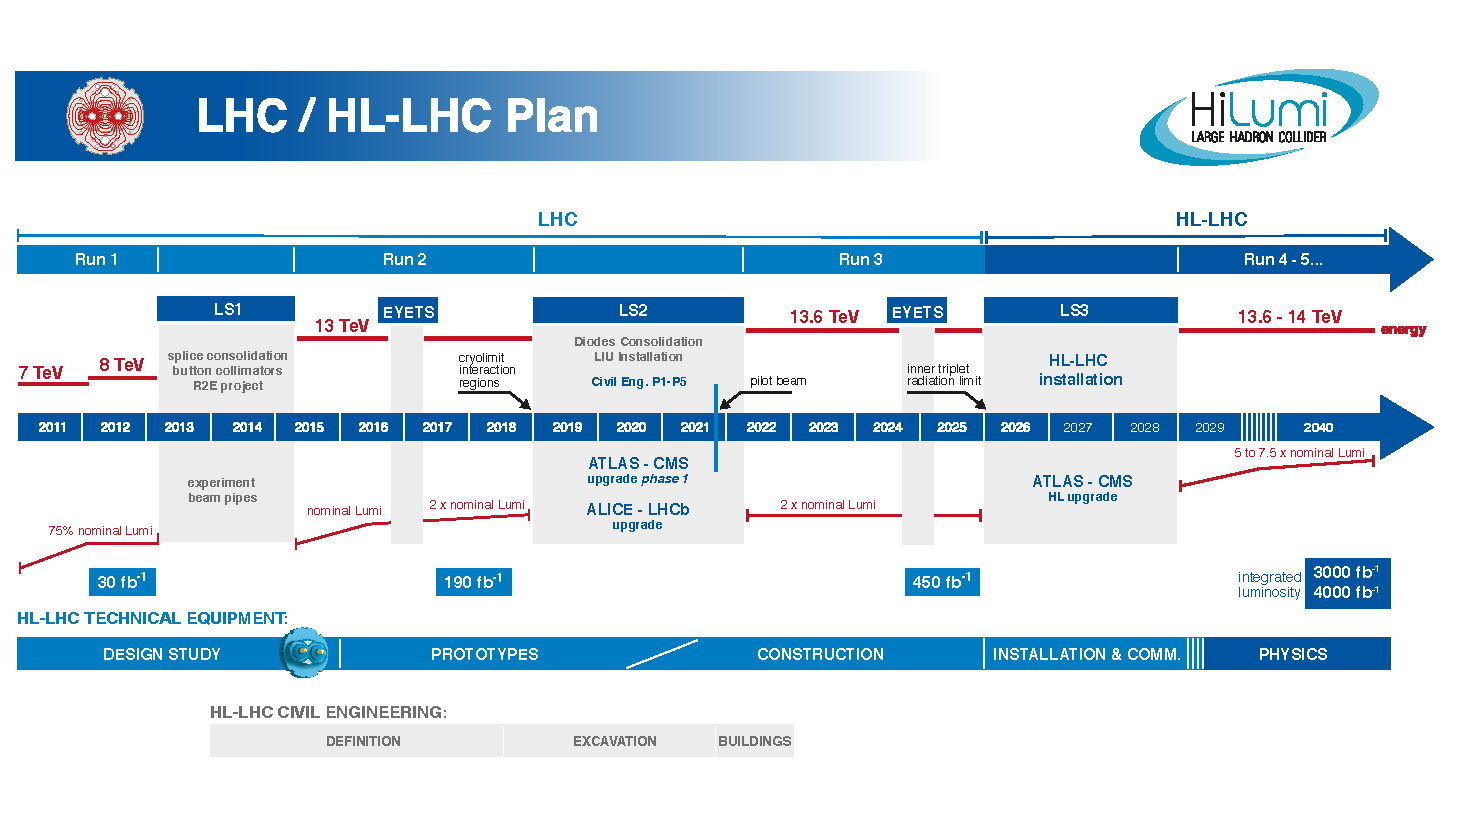
\includegraphics[width=0.8\linewidth]{figures/experiment/HL-LHC_Janvier2022.pdf}
    \caption{The operation and upgrade timeline of the LHC as of April 2024.~\cite{hl-lhc-web}}
    \label{fig:lhc-timeline}
\end{figure}

\Cref{fig:lhc-timeline} shows the operation timeline of the LHC and its experiments. Run-1 of the LHC spanned the data-taking period from 2010 to 2012, where the collision energy ranged from 7 TeV to 8 TeV. Run-2 was the data-taking period between 2015 and 2018 at $\sqrt{s}=$13 TeV, providing the dataset used to perform the analysis described in this thesis. As of April 2024, the LHC is in the third year of its third run of data-taking, at 13.6 TeV. Starting 2026, the LHC and the experiments on it will go through a series of upgrades to prepare for the High-Luminosity era of the LHC~\cite{Aberle:2749422}, during which an unprecedented amount (3000 $fb^{-1}$) of collision data is expected to be collected between 2029 and 2040 by the experiments, pushing the intensity frontier of physics.

\begin{figure}[!ht]
    \centering
    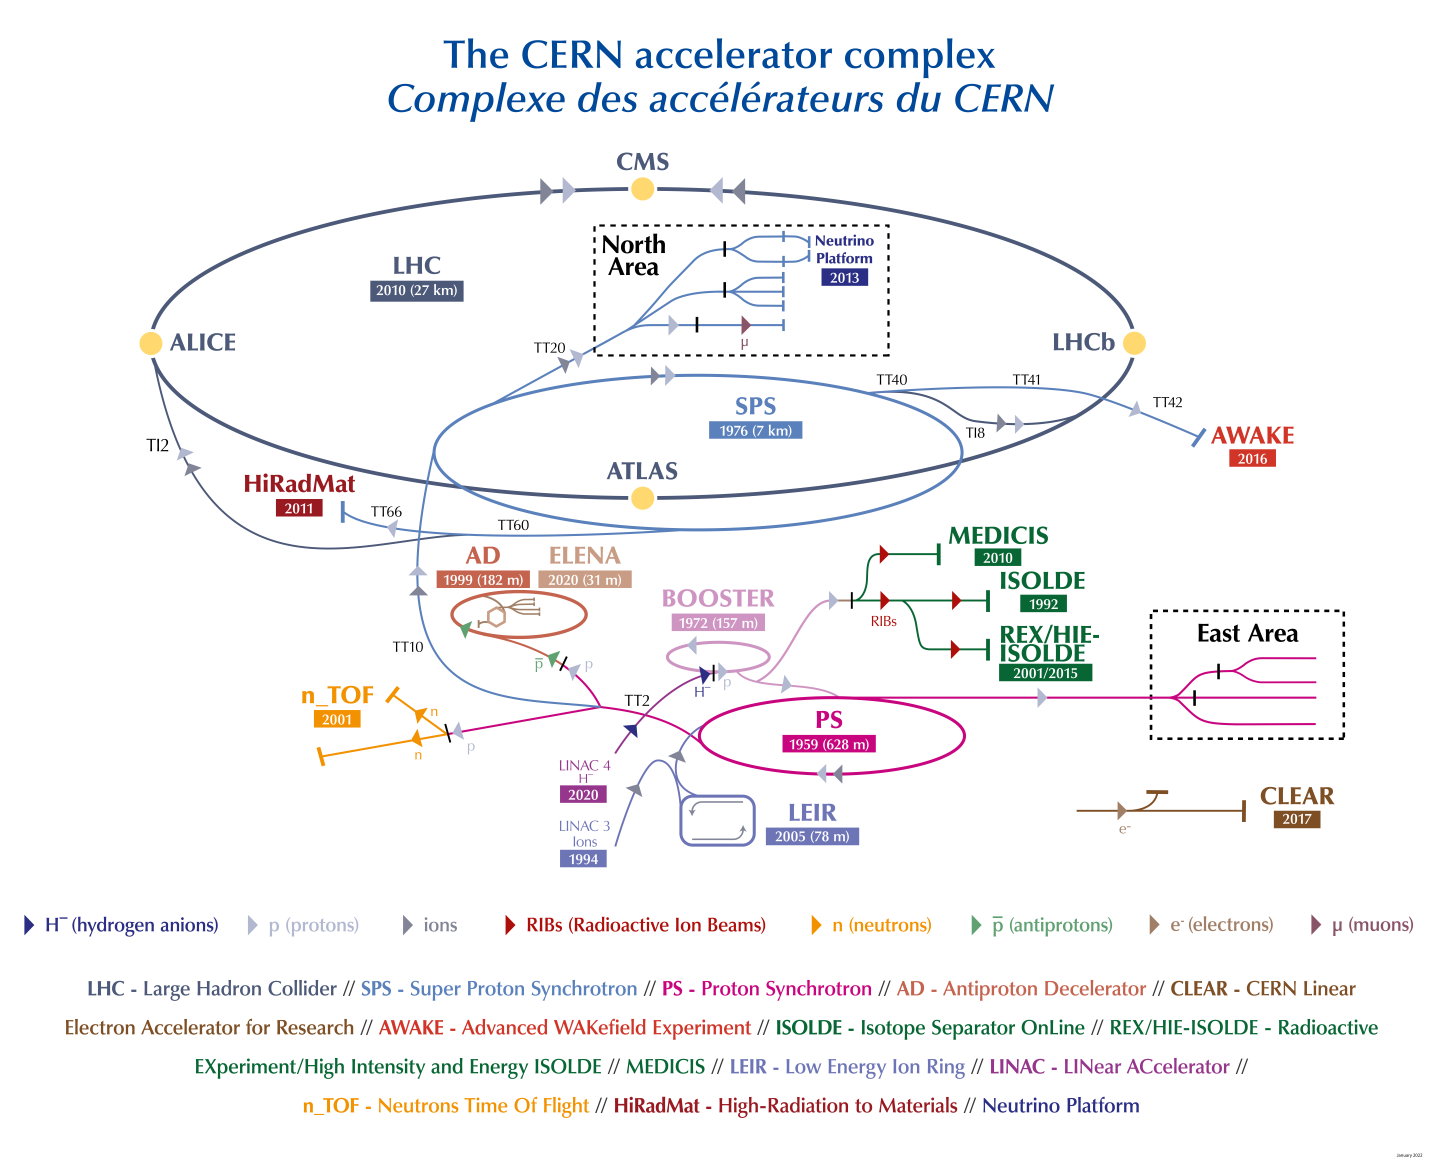
\includegraphics[width=0.8\linewidth]{figures/experiment/CCC-v2022.png}
    \caption{The CERN accelerator complex as of 2022.\cite{Lopienska:2800984}}
    \label{fig:cern-acc-comp}
\end{figure}

The acceleration of protons in the LHC happens in multiple steps, as shown in~\cref{fig:cern-acc-comp}. Protons are accelerated using the LINAC-4 (LINAC-2 during Run-1 and Run-2) machine to 50 MeV. The beam is then injected into the Proton Synchrotron Booster, followed by the Proton Synchrotron, which further accelerates the protons to 25 GeV. The pre-final stage is the injection into the Super Proton Synchrotron, where they are accelerated to 450 GeV, before being injected into the two main LHC rings. The beam in one pipe circulates clockwise while the beam in the other pipe circulates anticlockwise. Superconducting dipole magnets are used to create magnetic fields with a strength of about 8 T to further accelerate the protons to up to 6.8 TeV energies. 

The hadrons inside the LHC are accelerated using a radio frequency acceleration scheme~\cite{LHC}. The magnetic field inside the RF cavity osciallates, which affects only the protons with slightly different energies than the design energy arriving slightly early or late, causing them to either accelerate or decelerate. A direct consequence of this periodic acceleration is the bunch structure of beams. Under nominal operating conditions, each proton beam has 2808 bunches, with each bunch containing about $10^{11}$ protons. At full luminosity, the LHC uses a 25 ns bunch spacing corresponding to 40 MHz frequency. At the collision point at each of the 4 large experiments, the bunches are squeezed to about 20 $\mu$m sizes in a direction transverse to the beam to allow for greater chances of a proton--proton ($pp$) collision.

\section{The ATLAS Experiment} \label{sec:atlas}

A Toroidal LHC ApparatuS (ATLAS) experiment is one of the two general purpose experiments at the LHC, along with the CMS experiment. Situated at Point 1 of the LHC, ATLAS is designed to probe both $pp$ and ion--ion collisions. It is one of the largest detector system in the world with a length of 46 m, and a height and width of 25 m~\cite{ATLAS}. ATLAS is a cylindrically shaped experiment, built out of concentric detector sub-systems which provide a forward-backward symmetric coverage. Collisions happen at the center of this cylinder producing so-called \textit{outgoing particles}.

The sub-system closest to the interaction point (IP) is the Inner Detector (ID). The ID is responsible for reconstructing the trajectories of charged particles. These trajectories are in-turn used to identify the $pp$ collision of most interest, the \textit{hard scatter}, or the primary vertex (PV). It is also used to reconstruct secondary decays of non-prompt particles, or secondary vertices (SVs). ID is surrounded by the calorimeter system, which is used to measure the energy of all particles and stop them, except muons. The outermost detector layer of ATLAS is the Muon Spectrometer (MS) that identifies muons and also provides a secondary momentum measurement. \Cref{fig:atlas-layout} shows the layout of the ATLAS detector during Run-2.

\begin{figure}[!ht]
    \centering
    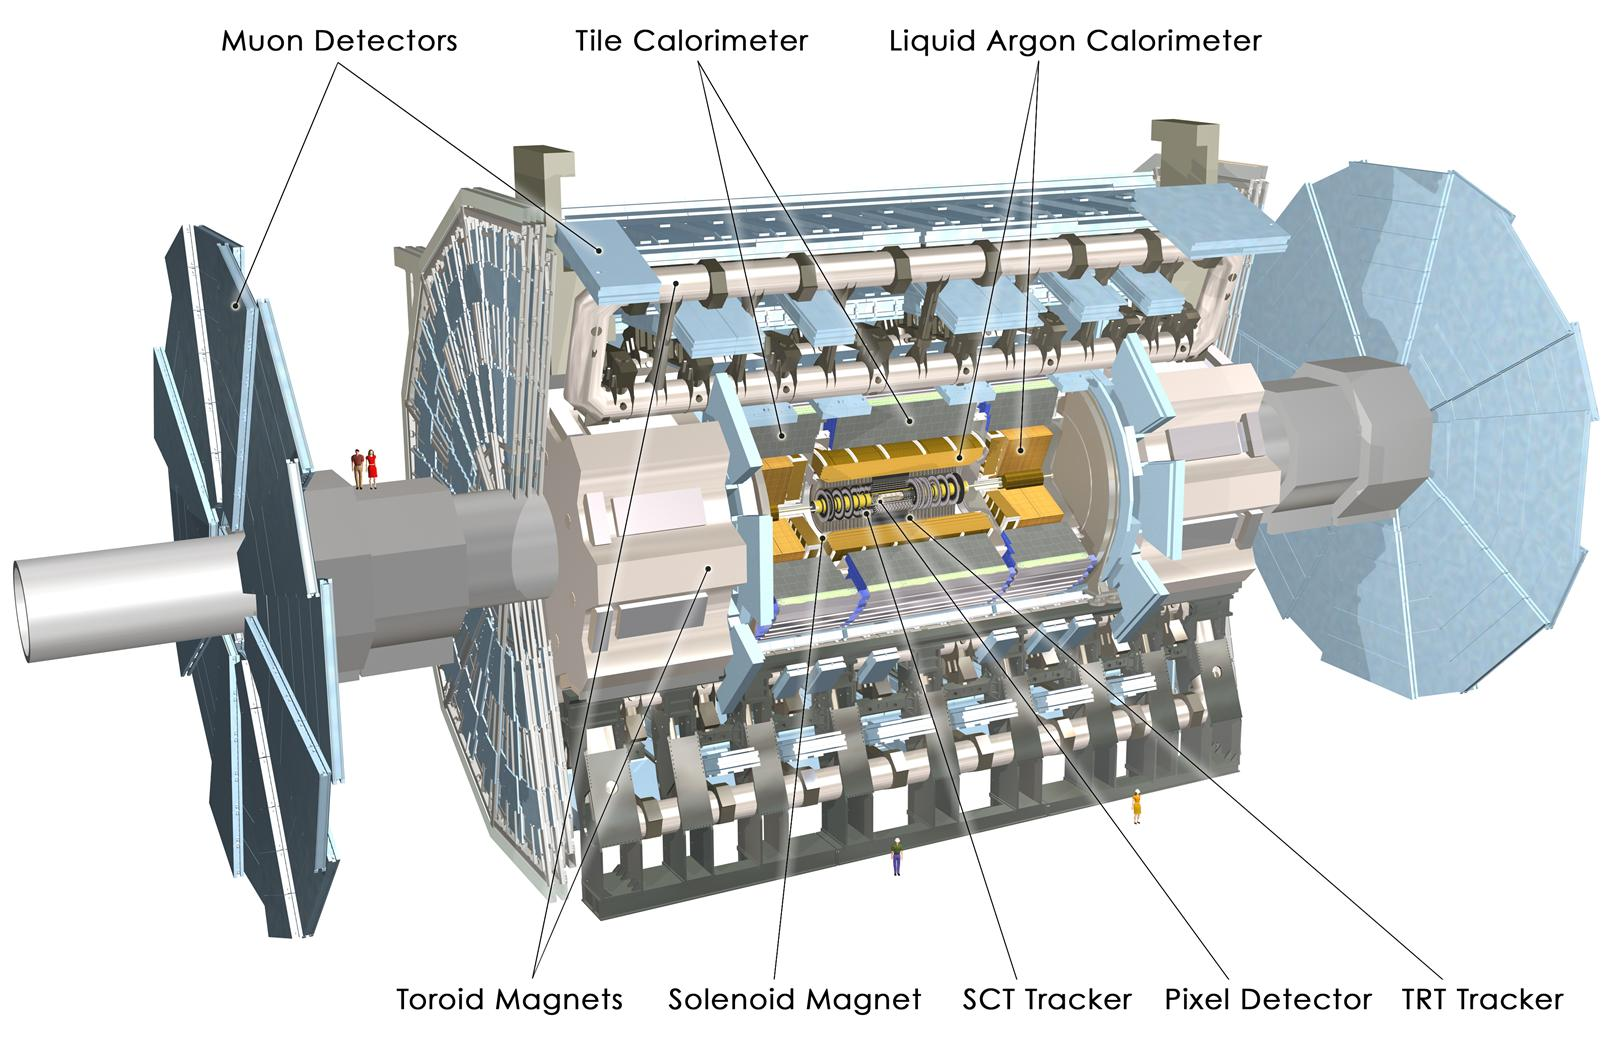
\includegraphics[width=0.8\linewidth]{figures/experiment/ATLAS-Run2.jpg}
    \caption{Layout of the ATLAS detector during the Run-2 data taking period.~\cite{Pequenao:1095924}}
    \label{fig:atlas-layout}
\end{figure}

ATLAS features a unique system of four large superconducting magnets. The ATLAS magnet system consists of:
\begin{itemize}
    \item a solenoid, which is aligned on the beam axis and provides a 2T axial magnetic field for the ID system;
    \item a \textit{central} toroid, and two \textit{forward} toroids, which produce a toroidal magnetic field of 0.5T and 1T for the muon detectors in the central and forward regions, respectively.
\end{itemize}

The exact magnetic field strengths and directions are measured using hall probes and the magnetic field map build out of this measurement iis used for reconstruction.

\subsection{ATLAS Geometry}

ATLAS follows a right-handed coordinate system to define the kinematics of objects in its measurements. The beamline defines the longitudinal $z$-axis, with the $xy$-plane transverse to it. The $x$-axis points towards the center of the LHC, and the y-axis points towards the Earth's surface. \Cref{fig:geo} illustrates the coordinate system used in ATLAS. 

\begin{figure}[!ht]
    \centering
    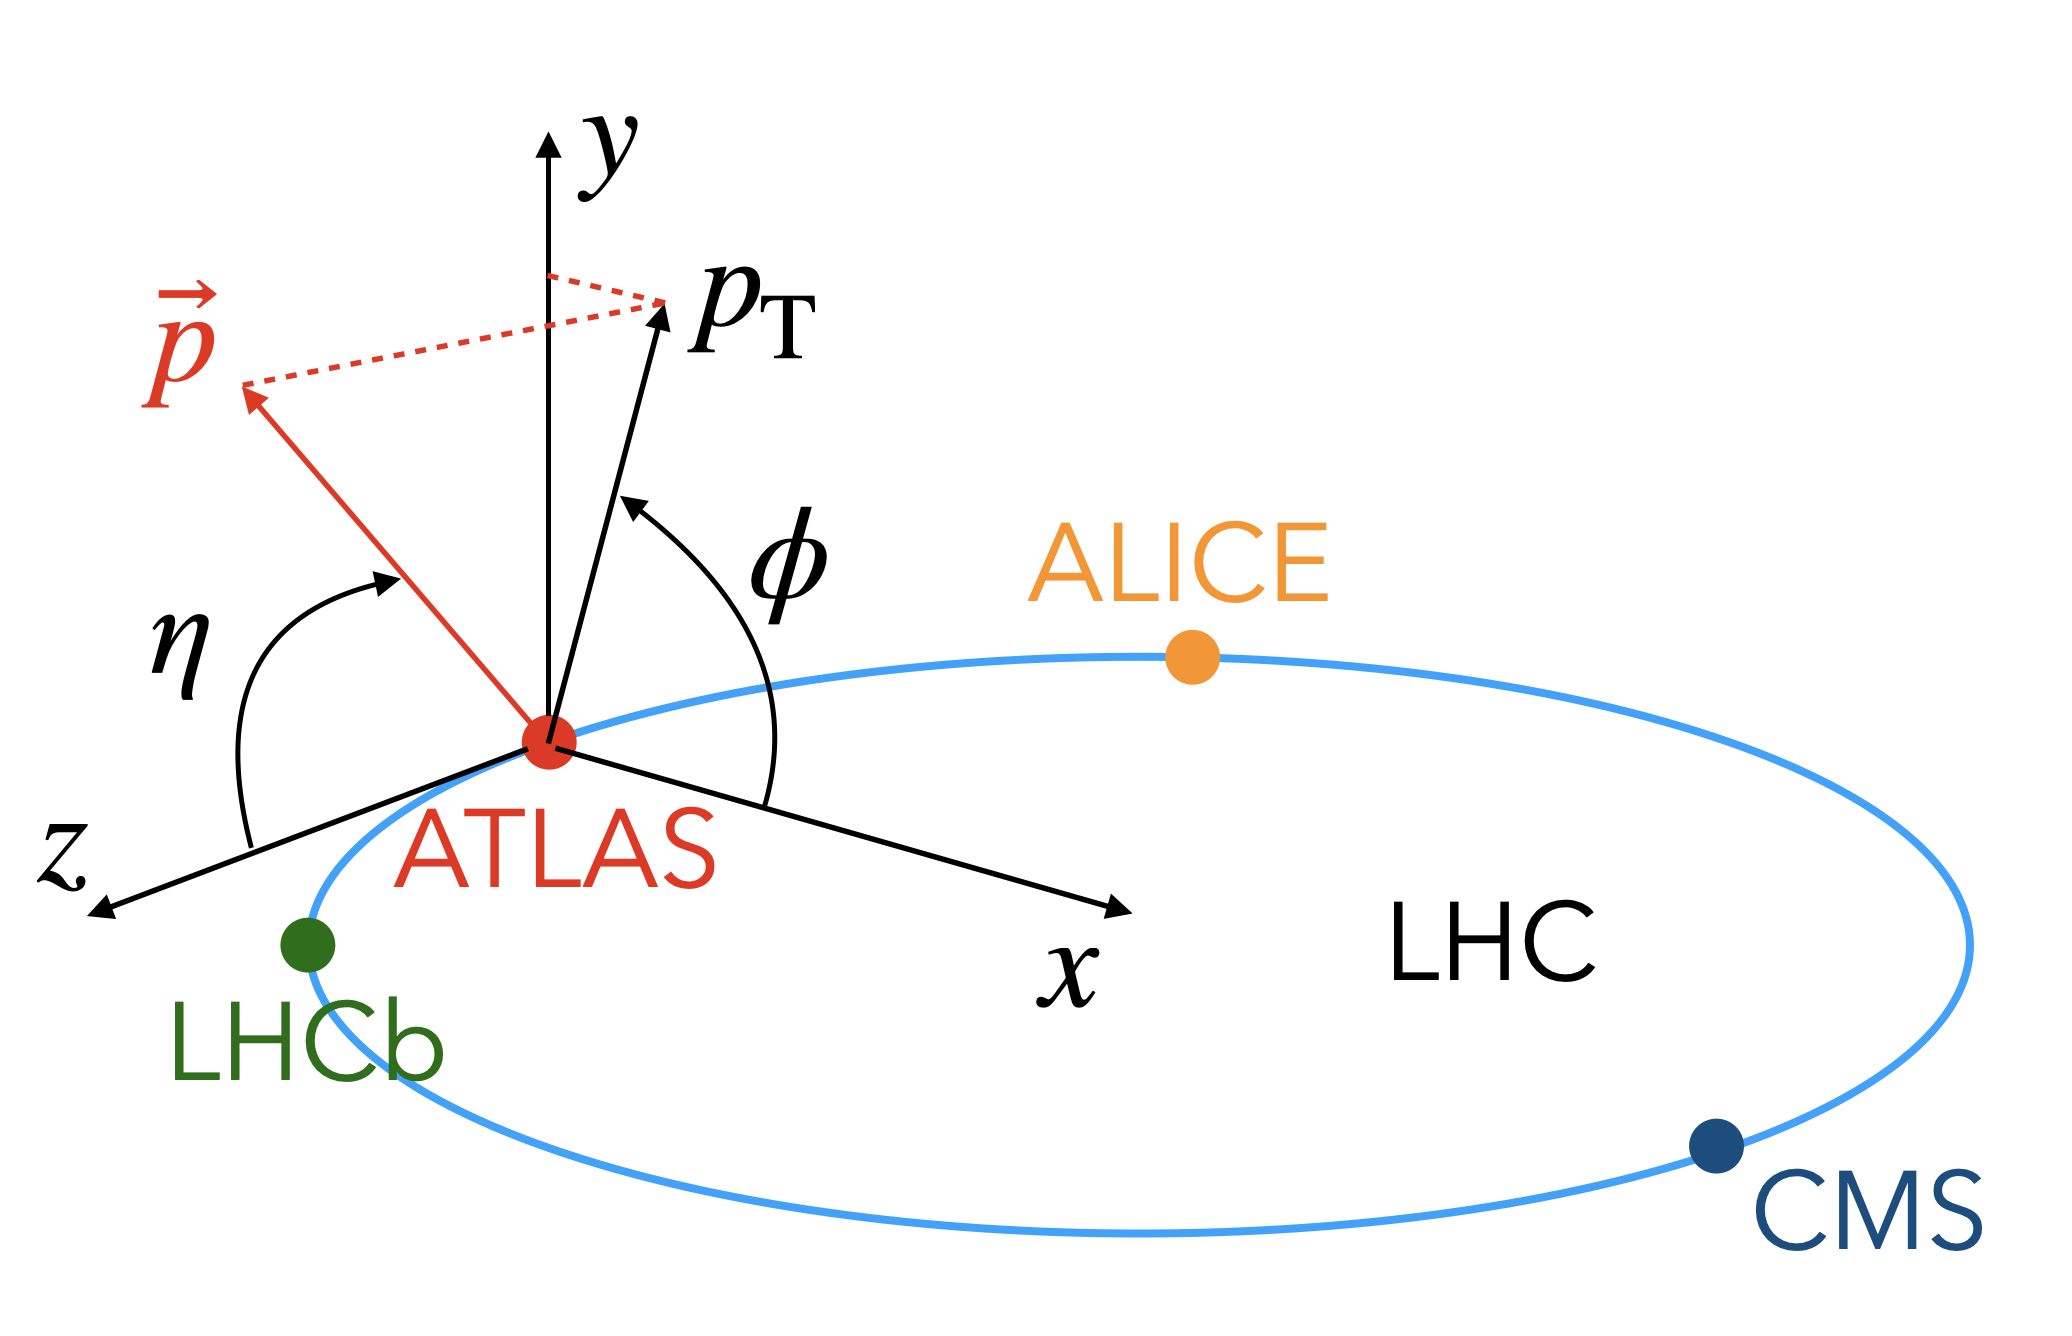
\includegraphics[width=0.7\linewidth]{figures/experiment/geometry.png}
    \caption{Geometry followed by ATLAS to describe directions and kinematics of particles.}
    \label{fig:geo}
\end{figure}

The angle in the transverse plane with respect to the $x$-axis is the azimuthal angle ($\phi$). The angle w.r.t. the beam direction is the polar angle ($\theta$), and is more commonly represented by the pseudo-rapidity ($\eta$) defined as:
\begin{equation}
    \eta = -\ln (\tan (\theta/2)),
\end{equation}

Angular distance is measured in units of $\Delta R = \sqrt{(\Delta\phi)^2 + (\Delta\eta)^2}$\footnote{The exact definition is $\Delta R = \sqrt{(\Delta\phi)^2 + (\Delta y)^2}$, where $y$ is the rapidity. At relativistic energies, $y\approx \eta$ and hence $\eta$ is generally used instead $y$.}. The projection of the momentum in the transverse plane, the transverse momentum (\pT), is defined as:
\begin{equation}
    p_\mathrm{T} = \sqrt{(p_x)^2 + (p_y)^2}.
\end{equation}

The ATLAS detector has a nearly full coverage in $\phi$, and a coverage in pseudo-rapidity up to $|\eta|$=4.9. The wall of the cylinder is also referred to as the \textbf{barrel}, and the side faces as the \textbf{endcaps}. The exact $\eta$ transition from barrel to endcap depends on the detector subsystem and shall be defined in relevant contexts throughout this chapter.

\subsection{Inner Detector}

The Inner Detector is the sub-system closest to the collision point.~\Cref{fig:inner-det} shows the cross-section of the inner detector system in the barrel. 

\begin{figure}[!ht]
    \centering
    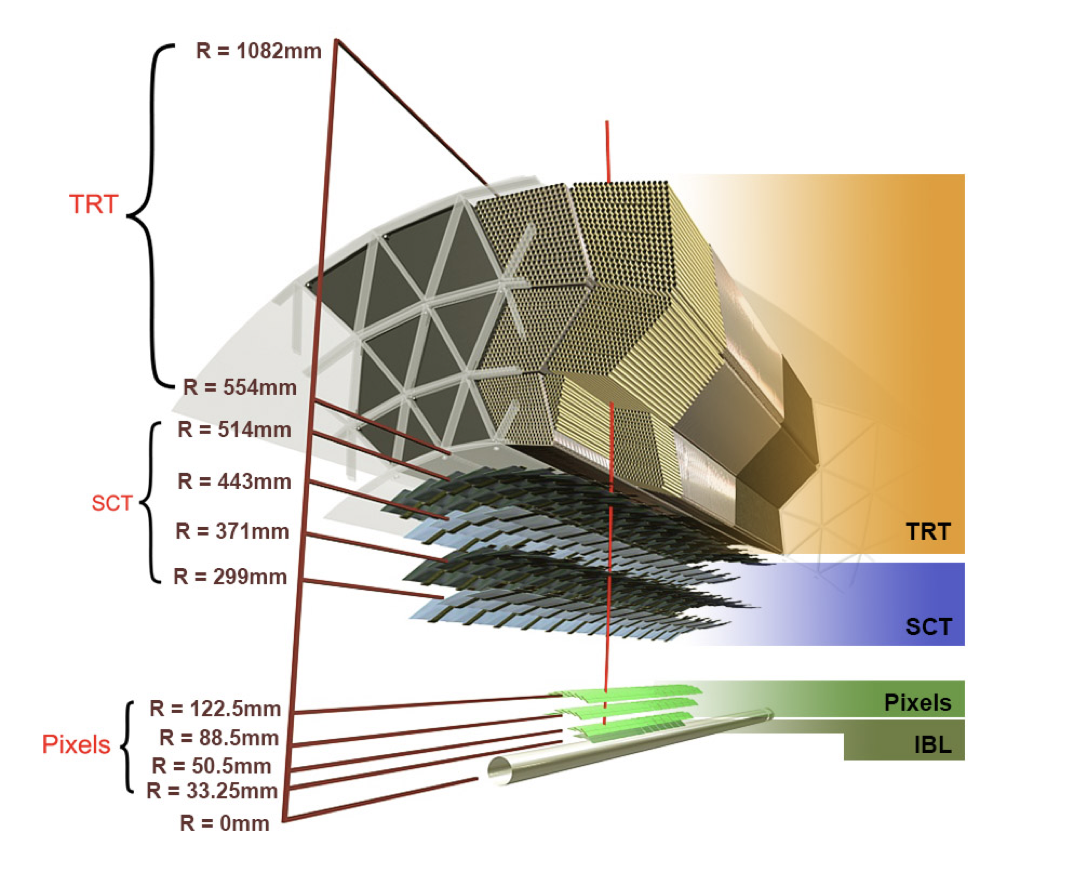
\includegraphics[width=0.8\linewidth]{figures/experiment/InnerDetector.png}
    \caption{Illustrative cross-section of the Inner Detector in the barrel region.~\cite{atlascollaboration2023software}}
    \label{fig:inner-det}
\end{figure}

The innermost layer is a pixel silicon detector, the Insertable B-Layer (IBL)~\cite{Capeans:1291633}, which was installed between Run-1 and Run-2 to help retain high reconstruction efficiency in high $pp$ collision density environments. The IBL is surrounded by three additional layers of pixel detectors. These four layers form the Pixel System. Having high-granularity detectors close to the collision point ensures efficient identification of the PV. The four layers of silicon micro-strip modules form the Semi-Conductor Tracker (SCT) system with a total of 4088 modules. Each barrel or disk provides two strip measurements from back-to-back modules glued at a stereo angle (40 mrad) which are combined to build a space-point. The outermost layer of the ID is the Transition Radiation Tracker (TRT) made out of approximately 300,000 thin-walled drift/straw tubes made out of kapton, each having a a gold-plated Tungsten wire 31 $\mu$m in diameter~\cite{CERN-LHCC-97-016}. The TRT is filled with an Argon-based gas mixture which is ionized by passing charged particles. \Cref{tab:id_chars} outlines the main characteristics of the different ID detectors in the barrel., The ID has a coverage roughly up to $|\eta|$=2.5 from the silicon detector layers, and up to $|\eta|$=2.1 from the gaseous detector.

\begin{table}[!ht]
    \centering
    \begin{tabular}{ccccc}
        \hline \hline
        Sub-detector & Active Element Size & Resolution & Hits in & Radius of the \\
         & $r-\phi \times z$ & [$\mu$m] & the barrel & barrel layers [mm] \\
         \hline
        IBL   & 50$\times$250 $\mu$m & 8$\times$40  & 1   & 33.25 \\
        Other Pixel & 50$\times$400 $\mu$m & 10$\times$115 & 3   & 50.5, 88.5, 122.5 \\
        SCT   & 80 $\mu$m          & 17            & 8   & 299, 371, 443, 514 \\
        TRT   & 4 mm               & 130           & $\sim$30 & 554-1082 \\
        \hline \hline
    \end{tabular}
    \caption{Main characteristics of the four ATLAS ID sub-detectors.~\cite{ATLAS-CONF-2014-047, ATL-INDET-PUB-2016-001}}
    \label{tab:id_chars}
\end{table}

\subsection{Calorimeters}
ATLAS consists of two calorimeter systems, the Electromagnetic Calorimeter (ECAL), and the Hadronic Calorimeter (HCAL), which are designed to detect electromagnetic and hadronic showers, respectively. When high energy electrons interact with dense material, they radiate photons via bremsstrahlung, and the photons in-turn produce electron pairs forming a shower. The shape and depth of the resulting shower depends on the incident energy of the electron, the resolution of which depends on the granularity of the calorimeter cells with added effects from the energy deposit and detector noise. The ECAL is designed to have a high granularity in the $\eta$ range of the ID for maximum photon and electron identification efficiency. Hadronic showers are, instead, intiated by a collision of an incident hadron against a nucleus. Such a collision leads to a decay with many hadrons and an excited nuclear state, which in turn decays decays into lighter hadrons. This cascade leads to a shower of hadrons which can interact via both, nuclear and electromagnetic reactions. Hence, the resulting showers are then measured in combination by the ECAL and HCAL. The ATLAS calorimeters can measure the kinetic energies of all particles that reach them, except for neutrinos and muons, since the former do not interact with the calorimeters at all and the latter leave $\sim$3 GeV energy in the calorimeter and pass through. \Cref{fig:calo} shows the layout of the calorimeters in the ATLAS detector. 

\begin{figure}[!ht]
    \centering
    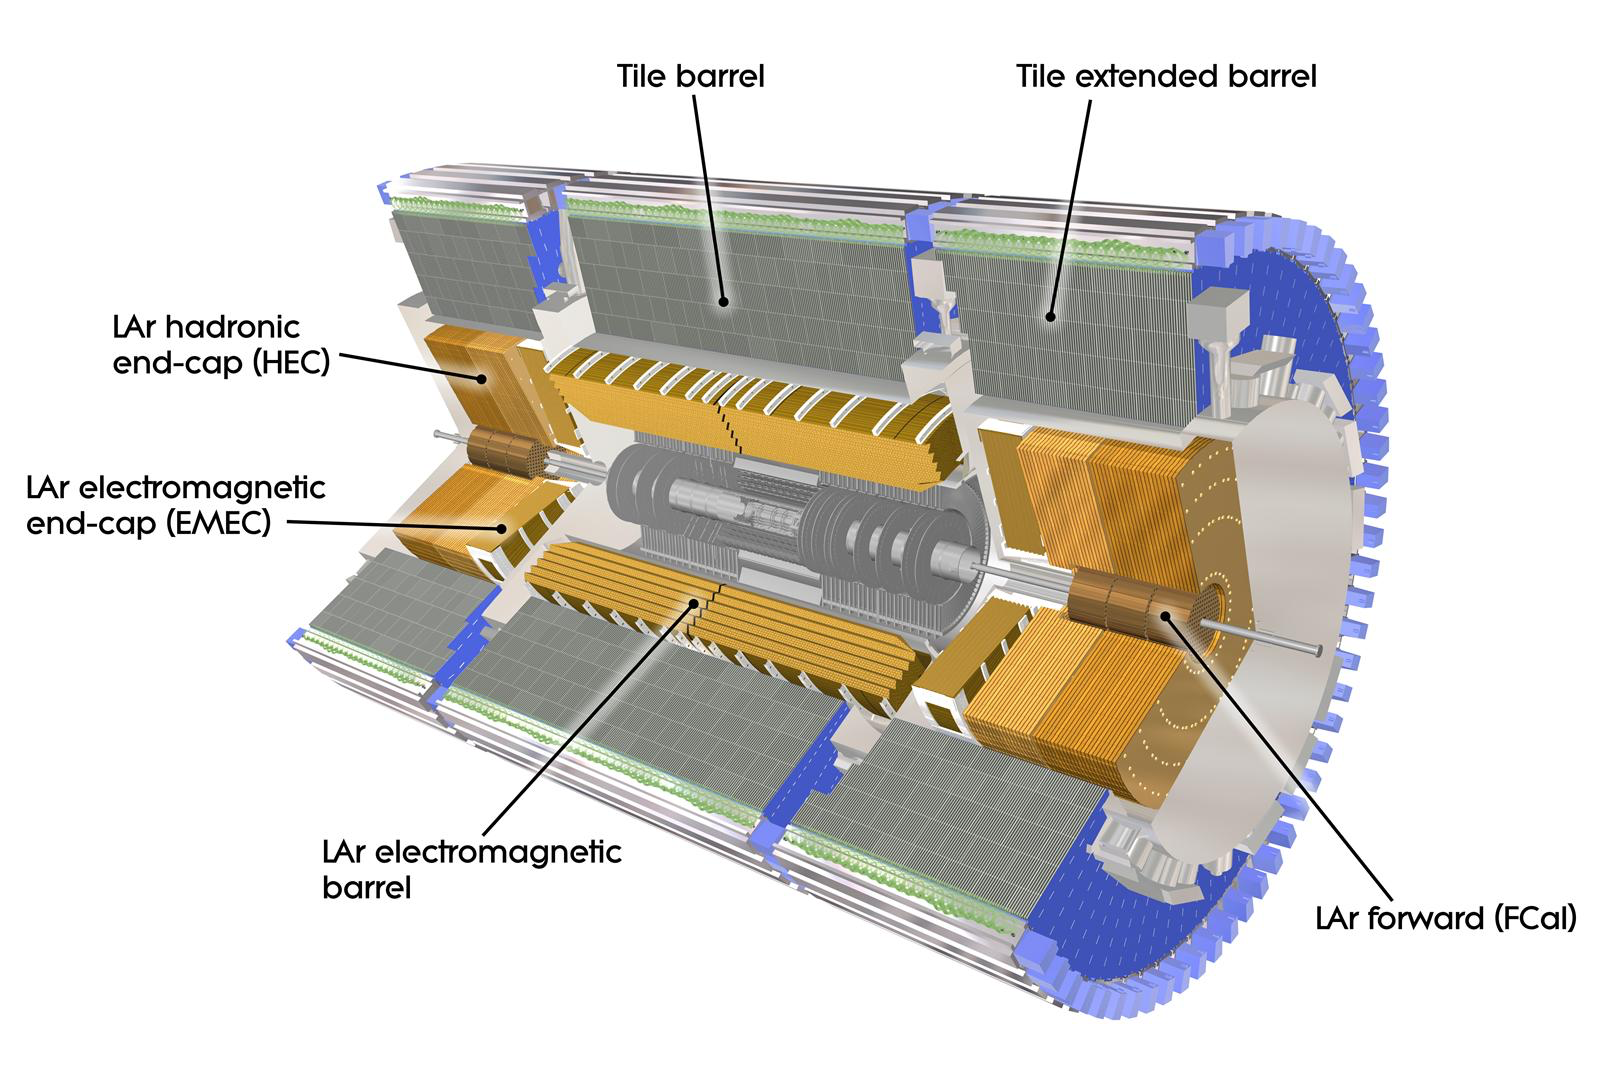
\includegraphics[width=0.8\linewidth]{figures/experiment/Calorimeters.png}
    \caption{Computer generator layout of the ATLAS Calorimeter subsystem.~\cite{Pequenao:1095927}}
    \label{fig:calo}
\end{figure}

The ECAL is divided into a barrel part ($|\eta|<$1.475) and two end-cap components (1.375$<|\eta|<$3.2). It is a hybrid lead-Liquid Argon (LAr) detector with accordion-shaped kapton electrodes and lead absorber plates over its full coverage. This geometry provides a full $\phi$ coverage. In the region of $|\eta|<$1.8, a presampler detector, made out of an active LAr layer of thickness 1.1 cm (0.5 cm) in the barrel (endcap) region, is used to correct for the energy loss of the electrons and photons upstream of the calorimeter.

The HCAL uses different detector technologies in different parts of ATLAS. In the barrel ($|\eta|<$1) and extended-barrel (0.8$<|\eta|<$1.7), steel is used as the absorber material and scintillating tiles as the active material. The Hadronic Endcap Calorimeter lies within 1.5$<|\eta|<$3.2 and uses a copper-LAr hybrid material. Finally, the LAr Forward calorimeter extends the range to 3.1$<|\eta|<$4.9, and serves as both an electromagnetic and hadronic calorimeter, with one layer of copper and two layers of tungsten, with LAr between the layers acting as the sensitive medium. 

\subsection{Muon System}

At the relativistic momentum values ($\mathcal{O}$(1-100) GeV/c) with which most muons are reconstructed in ATLAS, muons act as minimum-ionizing particles (MIPs). This causes them to lose only $\sim$3 GeV of energy in the calorimeter, and pass through all ATLAS detector systems. The ATLAS MS is a tracking subsystem providing a secondary momentum measurement (in addition to the measurement from the ID) for muons, and most importantly particle identification, since muons are the only charged particles that are not stopped by the calorimeters.

\begin{figure}[!ht]
    \centering
    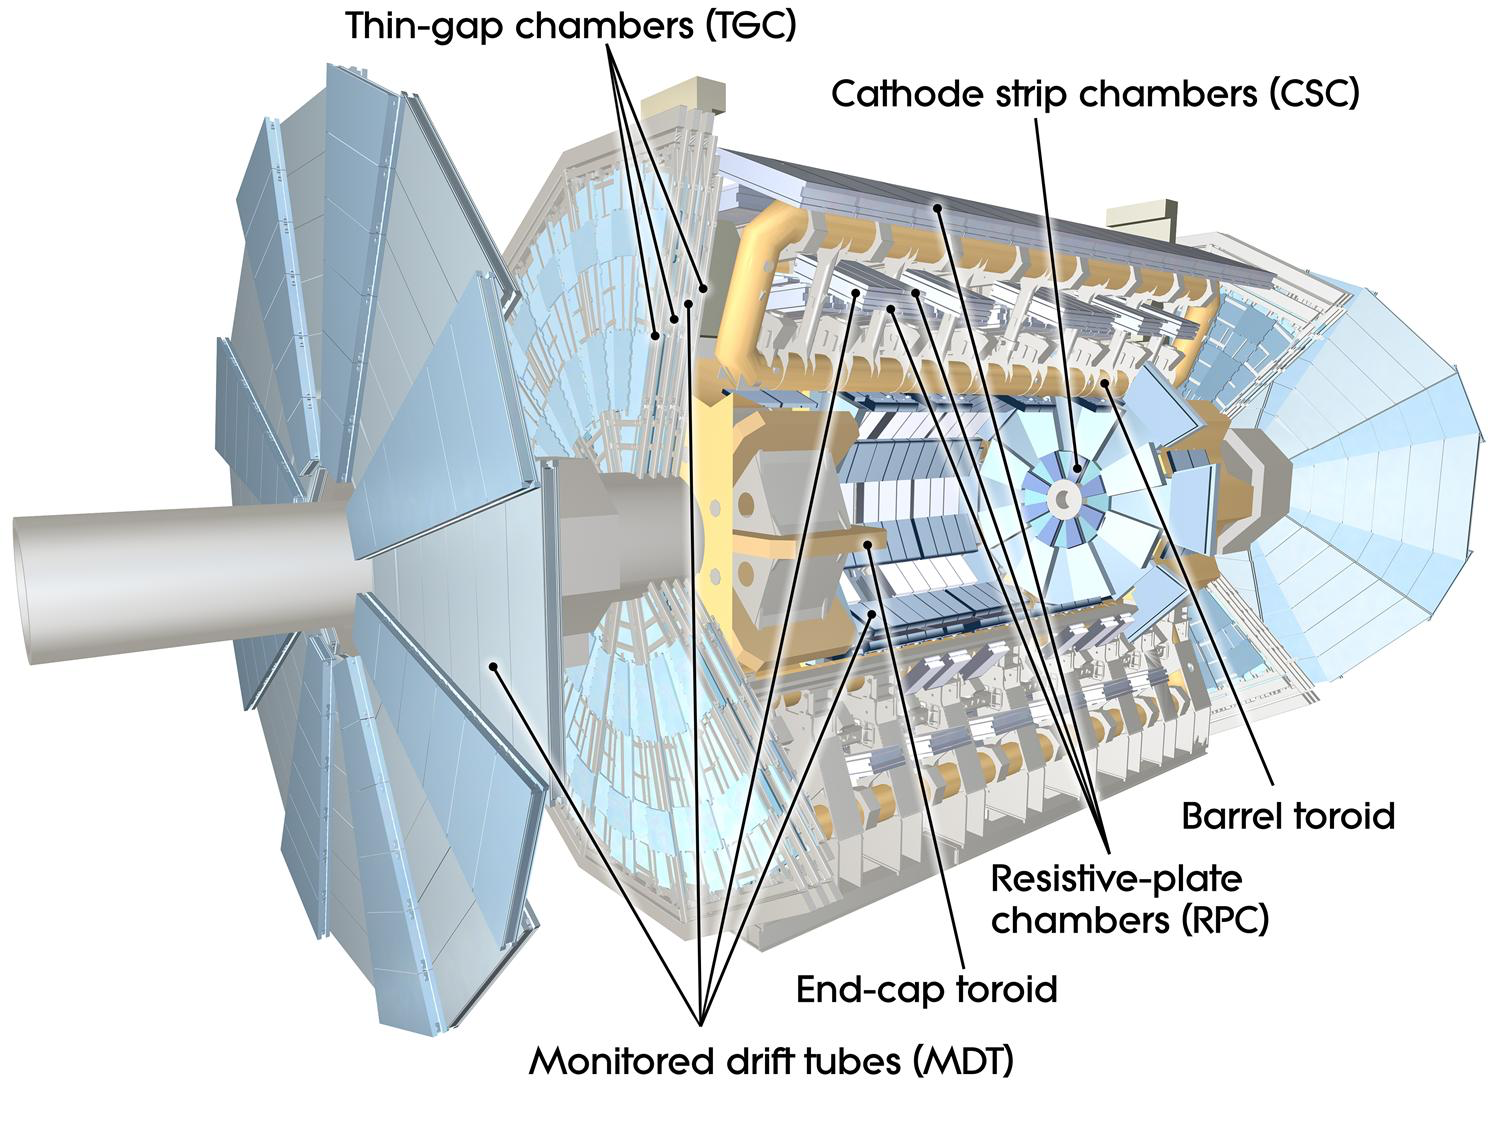
\includegraphics[width=0.7\linewidth]{figures/experiment/MuonSystem.png}
    \caption{Computer generator layout of the ATLAS Muon subsystem.~\cite{Pequenao:1095929}}
    \label{fig:ms}
\end{figure}

\Cref{fig:ms} shows the layout of the ATLAS MS. The MS consists of three concentric chamber layers in the barrel region and three disk layers in the endcap region. The toroid magnets provide the bending power in the MS, and the trajectory is reconstructed using signatures left in different sub-detectors. 

Over most of the $|\eta|$ range, a precision measurement of the track coordinates in the principal bending direction of the magnetic field is provided by the Monitored Drift Tubes (MDTs). MDTs have a coverage up to $|\eta|$=2.7 (2.0 for the innermost layer), and they use pressurised drift tubes with a diameter of 29.970 mm operating with an Ar/CO$_2$ mixture to collect muon hits. A central tungsten-rhenium wire with a diameter of 50 $\mu$m passes through the tubes. MDTs work on the same principle as the TRT, where drift circles left created by passing charged particles are measured by the electrodes to reconstruct their position. The technology and geometry allows for an average spatial resolution of 80 $\mu$m. Due to the relatively higher fluence of particles in the forward (2.0$<|\eta|<$2.7) region, a secondary set of detectors, Cathode Strip Chambers (CSCs), are used to maintain muon reconstruction efficiency. The CSC has perpendicularly running cathode and anode wires. A charged particle passing through the CSC knocks off electrons which flock to the anode and create a signal pulse in the cathode strips, giving a measurement of two position coordinates. The triggering of events (see~\cref{sub:trig}) in the MS is facilitated by Resistive Plate Chambers (RPCs) in the barrel and Thin Gap Chambers (TGCs) in the endcap. These detectors also provide a measurement of the second coordinate, which is the $\phi$ angle.~\Cref{tab:ms_systems} summarizes the coverage and functions of the ATLAS MS sub-detectors.

\begin{table}[!ht]
    \small
    \centering
    \begin{tabular}{ccc}
        \hline \hline
        MS Sub-detector & Coverage & Function \\
        \hline
        Muon Drift Tubes        & $|\eta|<$2.7 (innermost layer: $|\eta|<$2.0) & Precision tracking \\
        Cathode Strip Chambers & 2.0$<|\eta|<$2.7 & Precision tracking \\
        Resistive Plate Chambers & $|\eta|<$1.05 & Triggering, second coordinate \\
        Thin Gap Chambers & 1.05$<|\eta|<$2.7 & Triggering, second coordinate \\
        \hline \hline
    \end{tabular}
    \caption{$\eta$ coverage and function of the MS sub-detectors.}
    \label{tab:ms_systems}
\end{table}

\subsection{Trigger and Data Aquisition System} \label{sub:trig}
The LHC delivers a proton bunch every 25 ns, and each bunch is tightly packed with many protons which collide to give a large fluence of outgoing particles. The ATLAS experiment cannot record all of these events because of limitations imposed by the data-taking rate of the detector readout electronics and the storage and processing capacity of the computing infrastructure in place. Hence, a trigger system is used to record only the interesting physics events, where dedicated triggers are designed and optimized based on the targeted physics signatures.

The ATLAS Trigger and Data Acquisition (TDAQ) system is responsible for the so-called \textit{online}\footnote{\label{foot:offline} Online analysis refers to the (multi-)object reconstruction which takes place during data-taking for the purpose of trigger selection. Offline analysis refers to the full event reconstruction which happens downstream, after a decision has been made to retain the event.} processing, selecting and storing of events of interest for \textit{offline}\footref{foot:offline} analysis, and is shown diagrammatically in~\cref{fig:tdaq}. The TDAQ system runs in two levels: the hardware-based Level-1 (L1) trigger, and the software-based High Level Trigger (HLT). The L1 trigger runs on hardware computational elements thanks to their high parallelization capacity and processing speed. Latency requirements~\cite{ATLAS_TDAQ} imposed by the rate of collisions also require that the first level of processing happen within the cavern, since light is not fast enough to carry the data outside the cavern before the next event occurs. The HLT, on the other hand, can afford slower speeds thanks to the reduced throughput coming out of L1, and allows for the combination of event information from different parts of the detector~\cite{ATLAS_TDAQ}. In the HLT, a typical reconstruction sequence makes use of dedicated fast trigger algorithms to provide early rejection, followed by more precise and more CPU-intensive algorithms that are similar to those used for offline reconstruction to make the final selection~\cite{ATLAS_TDAQ}.

\begin{figure}[!ht]
    \centering
    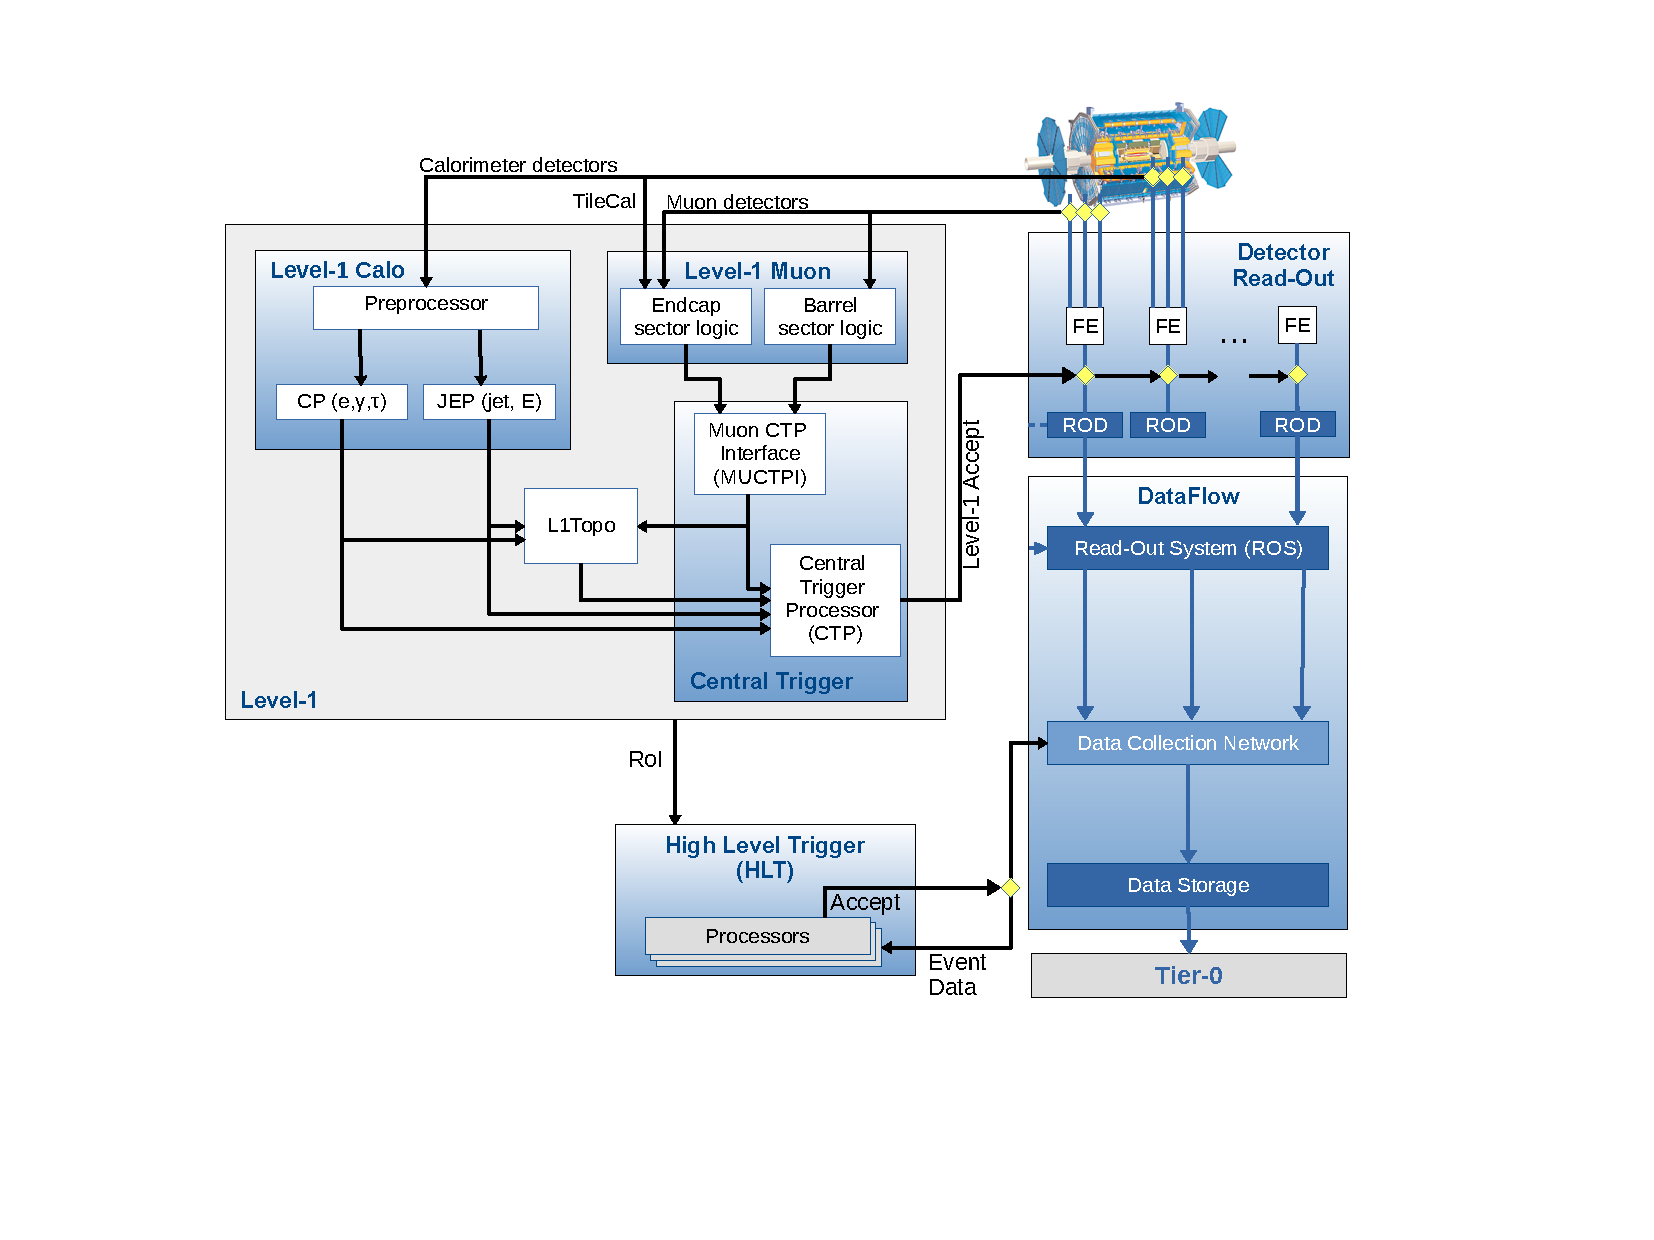
\includegraphics[width=0.7\linewidth]{figures//experiment/TDAQSystem.pdf}
    \caption{Schematic of the ATLAS Trigger and Data Acquisition System in Run-2. (Figure adapted from~\cite{ATLAS_TDAQ})}
    \label{fig:tdaq}
\end{figure}

The L1 uses information from the calorimeter and muon detectors~\cite{ATLAS_TDAQ}. The L1 calorimeter trigger takes signals from the calorimeter detectors as input while the L1 muon trigger uses hits from the RPCs (in the barrel) and TGCs (in the end-caps). To reduce the rate in the endcap region of particles not originating from the interaction point, the L1 muon trigger applies coincidence requirements between the outer and the inner TGC stations, as well as between the TGCs and the tile calorimeter~\cite{ATLAS_TDAQ}.

The L1 trigger accepts events at a rate up to the maximum detector-readout rate of 100 kHz, down from the bunch crossing rate of about 40 MHz. The HLT further reduces this physics output rate to an average of 1.2kHz. 

Combined with the average size of a physics event, the average physics throughput to data storage comes to 1.2 GB/s~\cite{ATLAS_TDAQ}. Once an event is accepted by the HLT, the data is sent to permanent storage for offline reconstruction at CERN’s computing centre.

\section{Particle Reconstruction} \label{sec:reco}

ATLAS can identify and reconstruct all known stable (except neutrinos) and some unstable particles. ~\Cref{fig:atlas-particles} illustrates the signatures left behind by particles passing through ATLAS. These signatures (such as hits or energy clusters) are \textit{stitched} together to identify the nature of the particle that left them and reconstruct its kinematics. This section discusses the standard reconstruction methods ATLAS uses to build so-called \textit{physics objects}.

\begin{figure}[!ht]
    \centering
    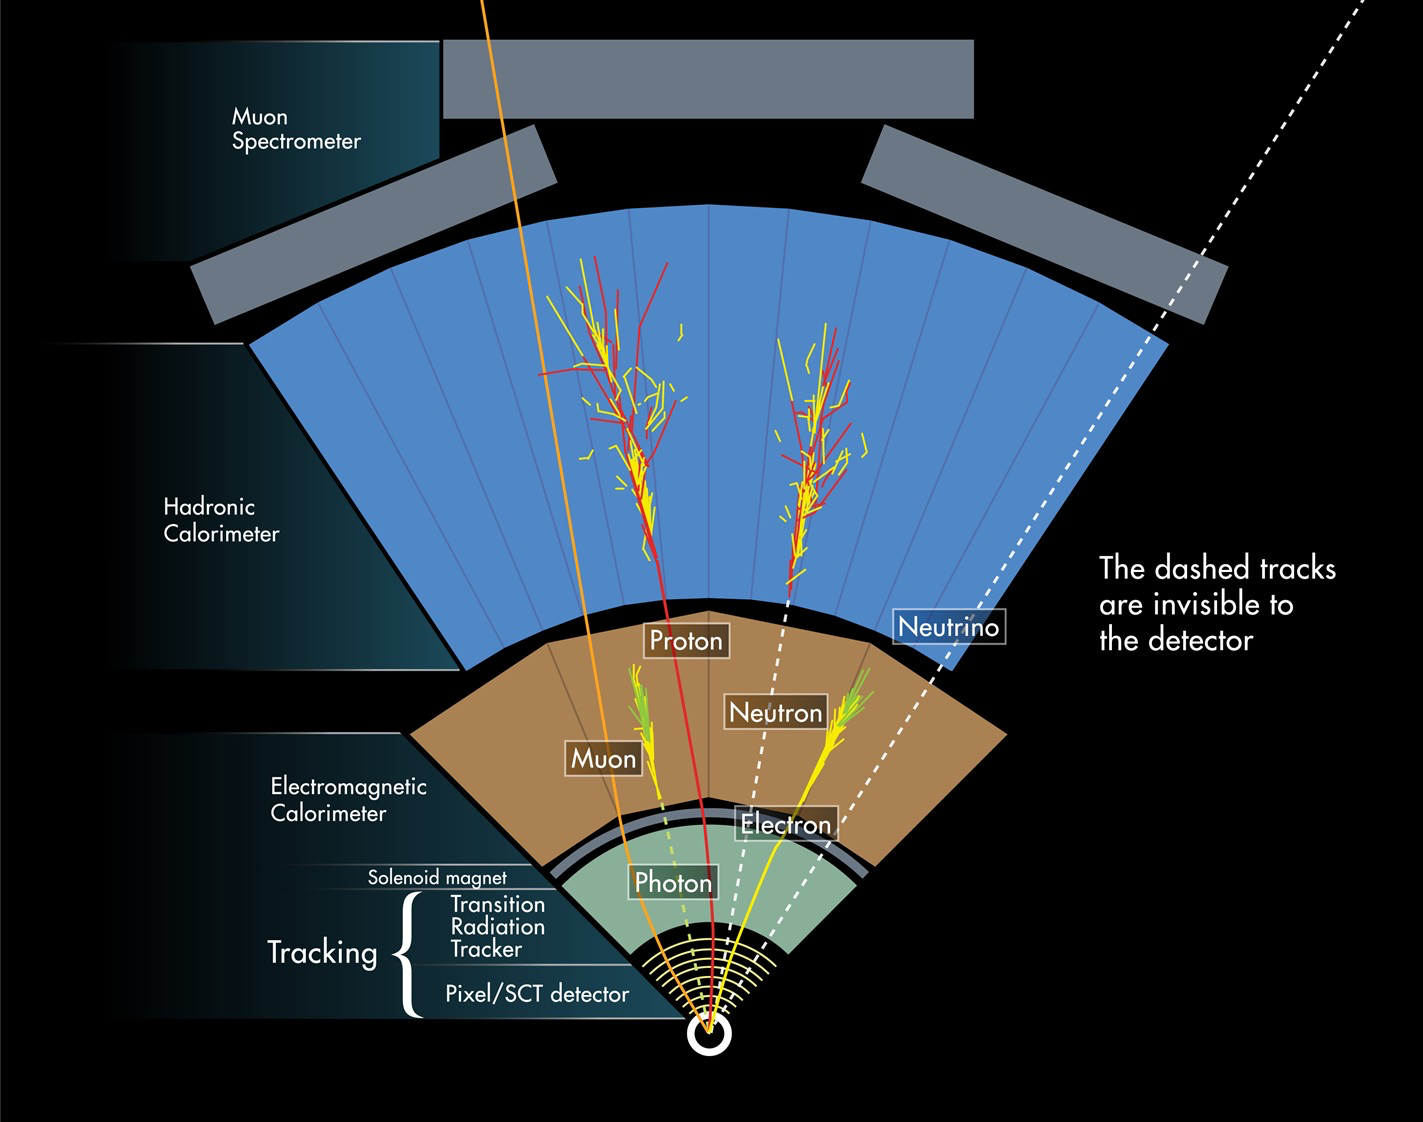
\includegraphics[width=0.8\linewidth]{figures//experiment/particlesATLAS.png}
    \caption{Simplied illustration of signatures left by stable particles in ATLAS.~\cite{Pequenao:1505342}}
    \label{fig:atlas-particles}
\end{figure}

As described in~\cref{sec:atlas}, the ATLAS sub-detectors are generally either \textit{trackers} (ID and MS), or calorimeters (ECAL and HCAL). Tracking refers to the identification of the series of hits that have been left behind by the a charged particle followed by the measurement of its trajectory using these hits. Calorimetry refers to the measurement of the direction and energy of a particle using clusters of calorimeter cells. The two methods provide complementary benefits, since the reconstructed momentum resolution from tracking gets worse with increasing particle momentum, whereas the energy resolution from calorimetry improves with increasing particle energy. The design inverse transverse momentum resolution~\cite{PERF-2015-09} for the ID is
\begin{equation}
    \sigma \left( \frac{1}{\pT} \right) \cdot \pT = 0.036\% \cdot \pT \oplus 1.3\% ,
\end{equation}
while the calorimeter energy resolution~\cite{PERF-2015-09} for single charged pions in the center of the detector is
\begin{equation}
    \frac{\sigma\left(E\right)}{E}=\frac{50\%}{\sqrt{E}}\oplus3.4\%\oplus\frac{1\%}{E},
\end{equation}
where energies and transverse momenta are measured in GeV.

\subsection{Tracks}

Tracks are reconstructed trajectories of charged particles using hits left behind by them in the ID system of ATLAS. For various reasons, track reconstruction is a critical step in the ATLAS analysis chain. Tracking gives a precise measurement of the momentum and the direction of charged particles, and provides an extrapolation of the trajectory to the IP, where a particle is nominally expected to originate from. 

\begin{figure}[!ht]
    \centering
    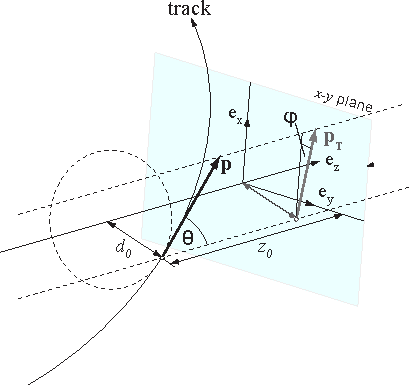
\includegraphics[width=0.6\linewidth]{figures/experiment/trackCoordinates.pdf}
    \caption{The parameters used to represent the helix trajectory of a charged particle with respect to the beamspot reference.~\cite{trk-tutorial-web}}
    \label{fig:track-coords}
\end{figure}

As shown in~\cref{fig:track-coords}, tracks are described by 5 helix parameters in a representation around the proton beam perigee (the ATLAS $z$-axis) with the reference point at the average measured beamspot position. Two of the parameters are the transverse ($\boldsymbol{d_0}$) and longitudinal ($\boldsymbol{z_0}$) impact parameters, defined as the transverse and longitudinal coordinate of the single point of closest approach transverse to the reference point. The other three parameters are the azimuthal ($\boldsymbol{\phi}$) and the polar ($\boldsymbol{\theta}$) angles of the track momentum at the reference point, and the ratio ($\boldsymbol{q/p_\mathrm{T}}$) of the charge of the reconstructed track divided by the magnitude of its momentum projected orthogonal to the magnetic field.

Track reconstruction happens in several steps, and in two \textit{passes}. The first pass, or \textit{inside-out} reconstruction, is the primary tracking method where the track finding is initiated in the pixels and SCT and then and TRT hits are added. The secondary pass, or \textit{outside-in} reconstruction, starts from the TRT and expanded to the silicon sub-detectors. The secondary pass aims at reconstructing tracks which start away from the IP using hits left behind after the primary pass. Specifically, it is designed to recover tracks from $\gamma \to e^+e^-$ conversions, and hence track reconstruction is only attempted in regions of interest determined by deposits in the ECAL. In the first step for both passes, hits from physically adjacent channels in the pixel and SCT sub-detectors are combined to form 3D clusters. These clusters are expected to be left behind by a single charged particle. In the TRT, drift circles are formed from the measured drift times of the gas by a charged particle. 

For the primary pass, seeds are formed using triplets of space-points either in the pixel or SCT, and a combinatorial Kalman filter~\cite{FRUHWIRTH1987444} is used to extend these seeds within a narrow search window based on an expected trajectory of the charged particle. An ambiguity resolution step follows which aims at partially resolving shared hits between track candidates, and a global $\chi^2$ minimizing fit is performed to obtain a high-precision track parameter estimate. Finally, an extension to the TRT sub-detector is performed where compatible TRT hits are added before performing a final $\chi^2$ minimizing fit.

Seeding for the secondary pass is triggered by segments of hits in the TRT compatible with the ECAL deposits, and doublets of space-points are constructed for the seeds instead of triplets. A similar Kalman filter based extension followed by ambiguity resolution and $\chi^2$ fit is performed, concluding with an extension to TRT.~\Cref{fig:track-steps} summarizes the steps used in the track reconstruction for both the primary and back-tracking passes in ATLAS.

\begin{figure}[!ht]
    \centering
    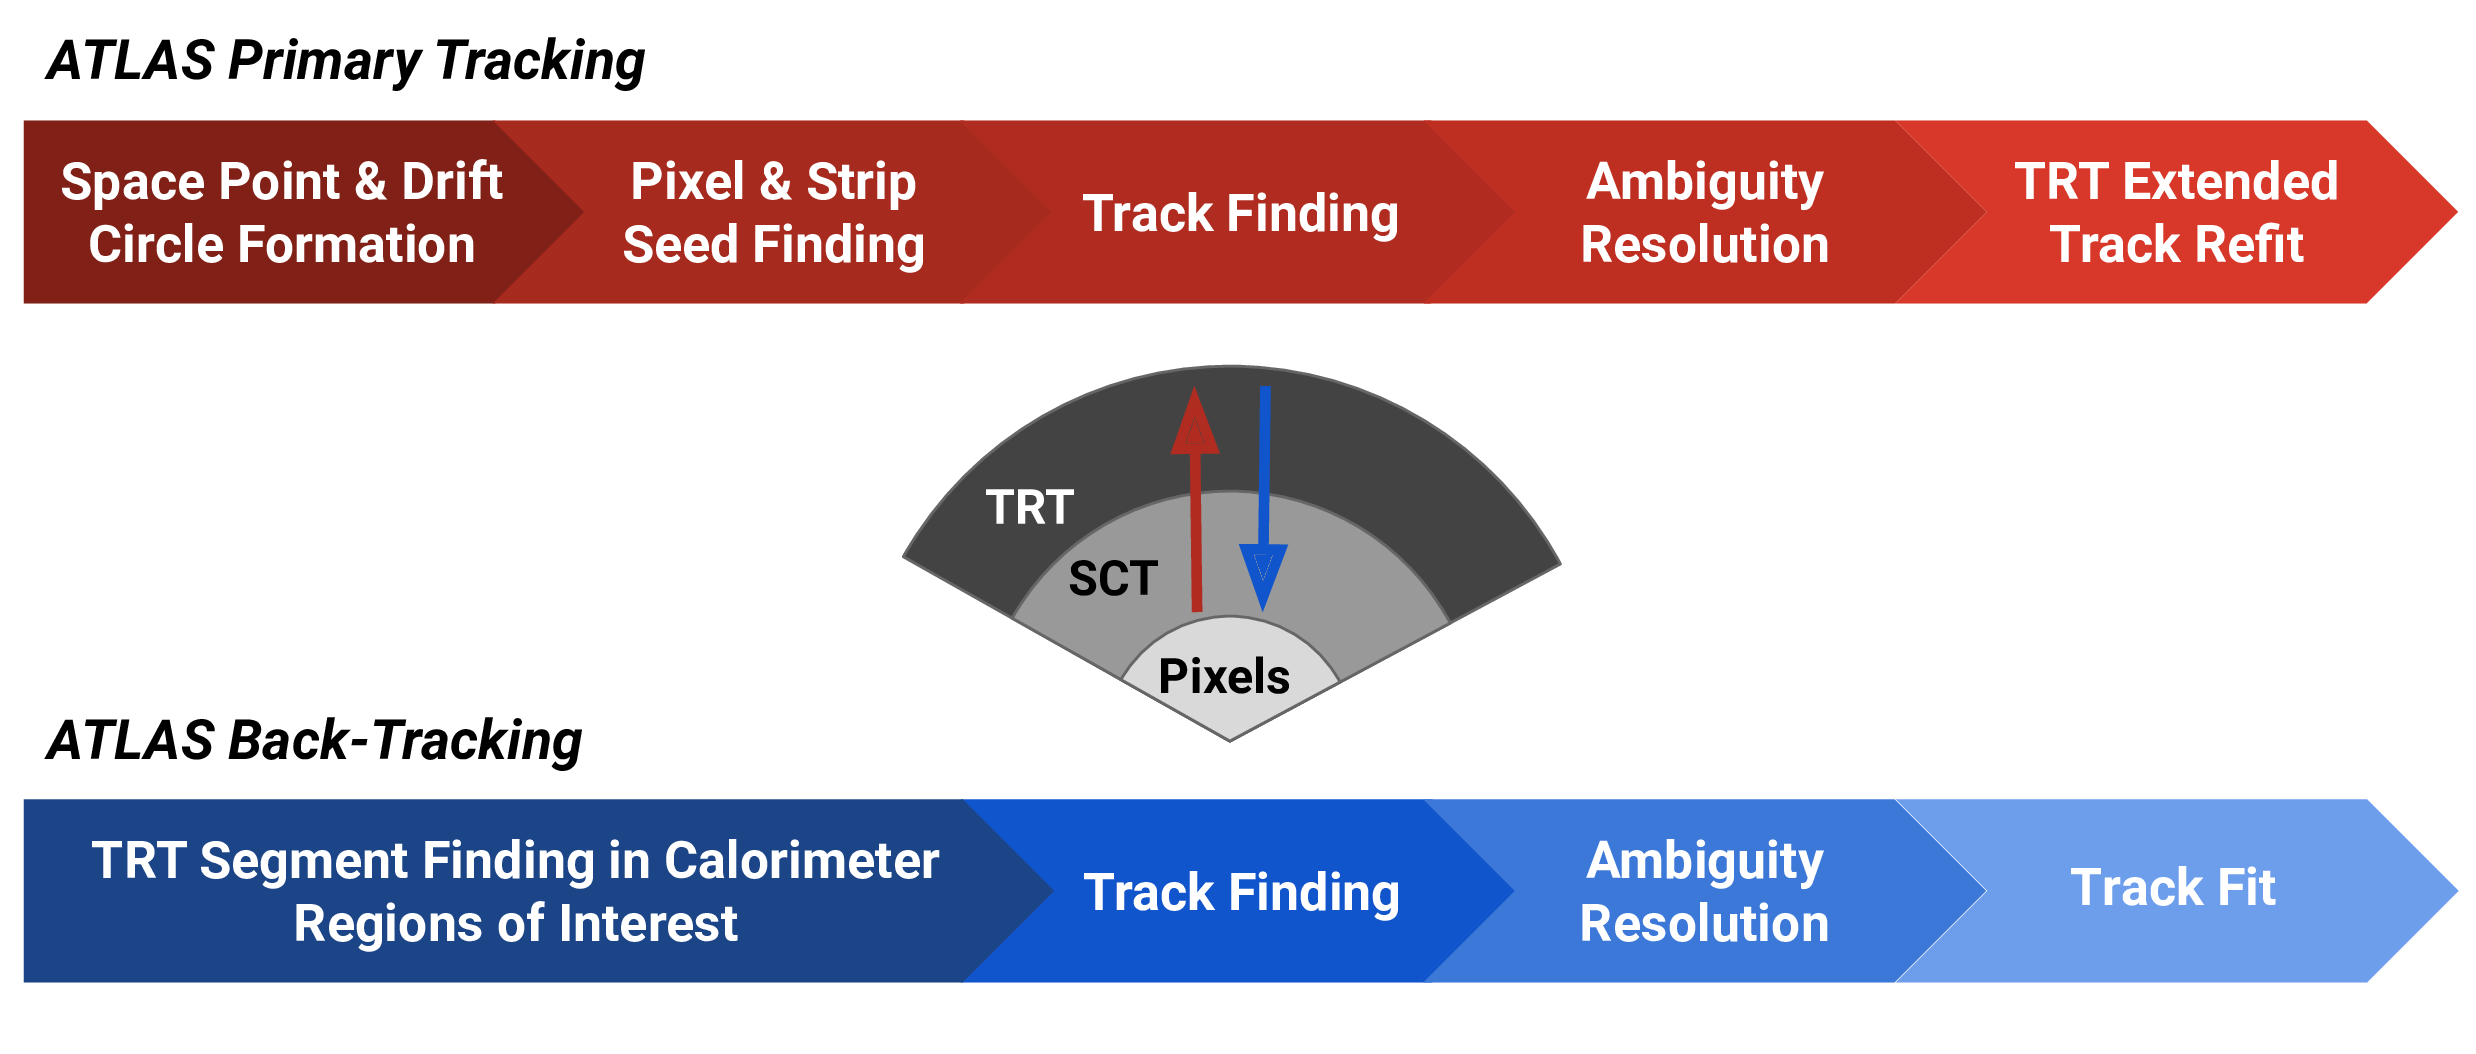
\includegraphics[width=0.8\linewidth]{figures//experiment/trackingSteps.png}
    \caption{Simplified overview of the primary tracking chain and secondary back-tracking chain used in ATLAS ID track reconstruction. The primary reconstruction runs from inside-out, starting from silicon space-points in the innermost Pixel and SCT subdetectors. The secondary back-tracking chain runs from outside-in, seeded from leftover TRT hits within electromagnetic calorimeter regions of interest.~\cite{atlascollaboration2023software}}
    \label{fig:track-steps}
\end{figure}

Given the high (and increasing) \textit{pileup} in ATLAS, the precise reconstruction of the multiple interactions and the accurate identification of the collision of interest (generally speaking, there's only one collision of interest) are extremely important for physics analyses. The locations of these interactions are determined using an adaptive multi-vertex fitter~\cite{Waltenberger_2007}. For most physics analyses in ATLAS, the PV is chosen as the vertex with the highest $\boldsymbol{\Sigma p_\mathrm{T}^2}$, where the sum is over all the tracks attached to the vertex.

\subsection{Large-Radius Tracking}
The two standard tracking passes in ATLAS, primary and back-tracking, are highly efficient in reconstructing tracks from most physics signatures, except those from LLPs. The primary pass doesn't cover tracks that do not originate from the primary $pp$ collisions, and the secondary pass is limited in coverage from the ECAL driven region of interest determination. Hence, there is significant loss in reconstruction efficiency for signatures from LLPs decaying within the ID volume. To recover this efficiency, ATLAS deploys a dedicated large-radius tracking (LRT) pass with loosened IP pointing requirements on the tracks. 

The primary tracking pass imposes a strict cut on the track candidate's transverse impact parameter ($|d_0|\leq$5 mm) to satisfy pointing requirements to the PV. This cut is significantly relaxed ($|d_0|\leq$300 mm) in the LRT pass. The LRT pass only uses the hits left after running the primary and the secondary passes for track reconstruction which limits possible combinatorics. To counterbalance the effect of such a loosening, other cuts are made stricter which determine the quality of the reconstructed tracks, having a net positive balance between the reconstruction efficiency of tracks from LLPs and the rate of fake combination of hits reconstructed as tracks. Similar to the primary pass, LRT runs only in an \textit{inside-out} fashion, with the seeding step only making use of SCT space-points. Fewer holes\footnote{A hole is defined as a missing hit on an active detector module, which was expected to be present between the first and last hits based on the particle trajectory.} are allowed in LRT, and no double holes\footnote{A double hole is defined as two consecutive missing hits on active detector modules where both were expected between the first and the last hit based on the particle trajectory.} are allowed. Furthermore, the width of the window used for to search for modules for hits during seed extrapolation (road width) is much narrower in the LRT pass (5 mm vs 12 mm).~\Cref{tab:std-lrt-diff} summarizes the main differences between the reconstruction criteria of the primary tracking pass and LRT.


\begin{table}
    \centering
    \begin{tabular}{lcc}
        \hline \hline
        Selection Criteria & Primary (\textit{inside-out}) & LRT \\
        \hline
        max. $|d_0|$ [mm] & 5 & 300 \\
        max. $|z_0|$ [mm] & 200 & 300 \\
        min. \pT [GeV] & 0.5 & 1 \\
        max. $|\eta|$ & 2.7 & 3.0 \\
        max. silicon holes & 2 & 1 \\
        max. double holes & 1 & 0 \\
        max. holes gap & 2 & 1 \\
        road width [mm] & 12 & 5 \\
        seeding & Pixels and SCT & SCT only \\
        max. seeds per middle Pixel space-point & 1 & - \\
        max. seeds per middle SCT space-point & 5 & 1 \\
        \hline \hline
    \end{tabular}
    \caption{Most important selection criteria that differ between the inside-out primary tracking and LRT setups.~\cite{IDTR-2021-03}}
    \label{tab:std-lrt-diff}
\end{table}

\Cref{fig:track-reco-eff-HNL} shows the track reconstruction efficiency of muons or electrons for simulated long-lived Heavy Neutral Lepton (\mhnl = 10 GeV, \ctau = 10 mm) production events as a function of the true $|d_0|$ of the HNL decay products, which are two charged leptons (two electrons, two muons, or one electron and one muon) and a neutrino for the study in the plot. As expected, the efficiency from the standard tracking passes (in pink) fall sharply after $|d_0|=$5 mm, whereas the LRT pass recovers the loss to a very high degree (in blue). The slight dip in total efficiency after $|d_0|=$5 mm is due to the stricter requirements imposed on tracks in the LRT pass, as outlined in~\cref{tab:std-lrt-diff}.

\begin{figure}[!ht]
    \centering
    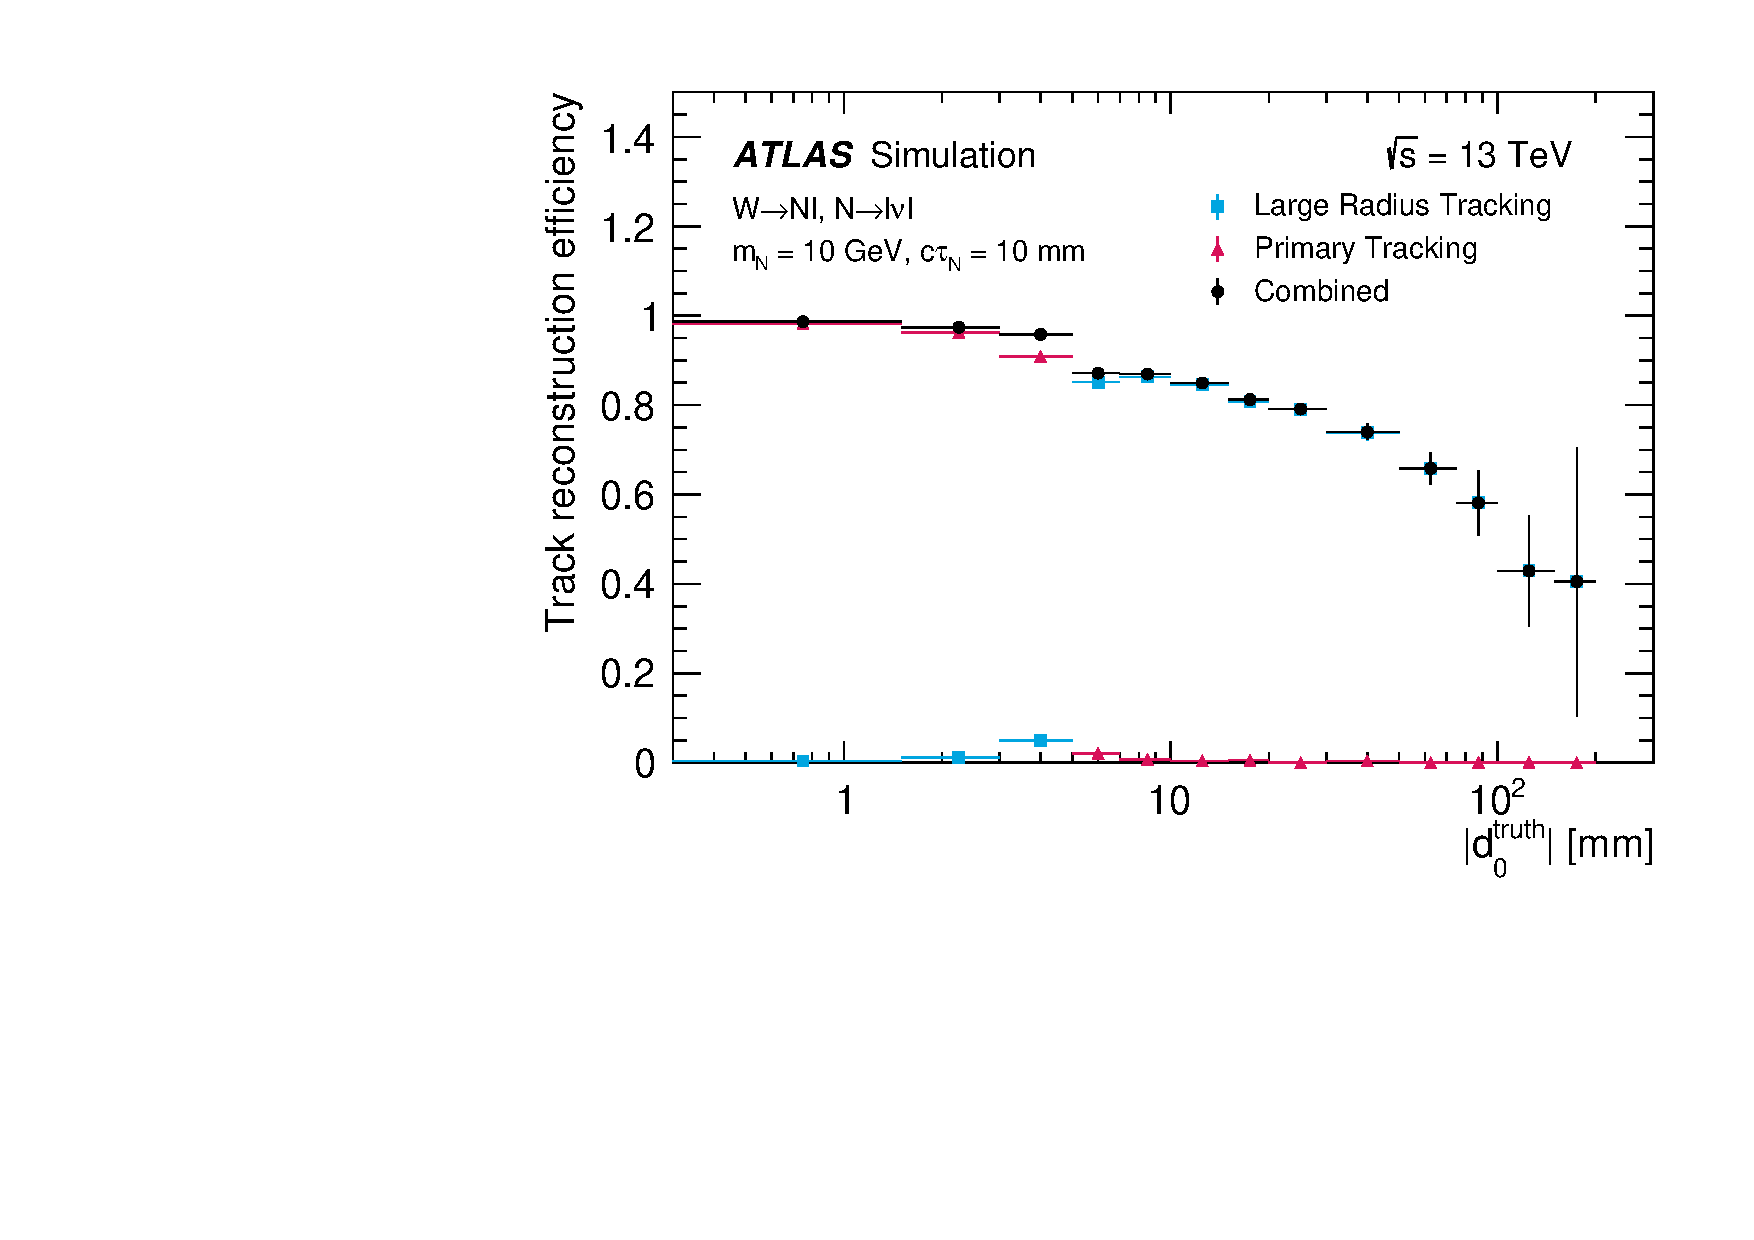
\includegraphics[width=0.8\linewidth]{figures//experiment/track-eff-HNL.pdf}
    \caption{Track reconstruction efficiency as a function of the true track $|d_0|$ for simulated Long Lived Heavy Neutral Lepton (\mhnl = 10 GeV, \ctau = 10 mm) production and decay events.~\cite{IDTR-2021-03}}
    \label{fig:track-reco-eff-HNL}
\end{figure}


\subsection{Muons}
Like track reconstruction, muon reconstruction also happens in several steps and in two passes. The primary reconstruction pass runs \textit{outside-in}, starting from hits in the MS followed by an attempted combination with ID tracks. The secondary reconstruction pass runs \textit{inside-out} attempting to recover muons with low \pT which do not leave clean tracks in the MS. The first step common to both passes is cluster formation, where signals from adjacent channels in the CSC are combined. Muons are not expected to leave hits in multiple drift tubes of the same layer. Straight line \textit{muon segments} are formed using a Hough transform in the MS in each of the tracking layers. ID tracks are pre-selected based on minimum silicon hit requirements, and are extrapolated to the inner surface of the MS to obtain their expected 3-momentum at the intersection point.

For the primary pass, segments from all MS layers are combined to form MS tracks. Seed segments are formed in the middle MS layer, and an extrapolation is done based on an assumed parabolic trajectory of the muon. An ambiguity resolution step follows to resolve tracks which share hits, and a global $\chi^2$ minimizing fit is performed to obtain the final MS track. MS tracks with $|\eta|<2.5$ are combined with ID tracks to improve the track-parameter resolution. ID tracks in a narrow angular window of compatibility wit the MS tracks are selected and combined with the MS track in a final global $\chi^2$ fit which also accounts for the energy loss of the muon in the calorimeter. MS information may be added or removed from the candidate based on this final fit quality. The primary pass yields three different types of muons:
\begin{itemize}
    \item \textbf{Combined (CB) muons} with a full MS track and a full ID track,
    \item \textbf{Silicon-associated Forward (SiF) muons} beyond $|\eta|=$2.5 which have an MS track associated with a "tracklet" consisting of only pixel hits, but not a full ID track, and
    \item \textbf{Standalone (SA) muons} with a full MS track but no associated ID track or hits.
\end{itemize}

While the primary pass reconstructs the majority of the muons used in ATLAS, a secondary recovery chain is run to recover low \pT muons and muons in regions where the MS lacks coverage. The reconstructions start using ID tracks and their extrapolation to the MS to estimate their momentum at the MS entrance, and three different types of muons are reconstructed in this pass:
\begin{itemize}
    \item \textbf{Segment-tagged (ST) muons} have a full ID track but do not have enough momentum to go beyond the first MS layer. A muon segment is required but is only used for PID, and no combined fit is attempted;
    \item \textbf{Calorimeter-tagged (CT) muons} have a full ID track and a corresponding deposit in the ECAL compatible with a deposit from a MIP. No information from the MS is used;
    \item \textbf{Inside-out combined muons} have a full ID track and muon segments, with their kinematics reconstructed using a full global $\chi^2$ fit. Such muons are useful in recovering muon reconstruction efficiency in the $|\eta|<0.1$ region, where half the sectors are not instrumented and hence an \textit{outside-in} approach fails.
\end{itemize}
~\Cref{fig:muon-types} illustrates the different types of muons reconstructed by ATLAS. SiF muons are omitted from the diagram for simplicity.

\begin{figure}[!ht]
    \centering
    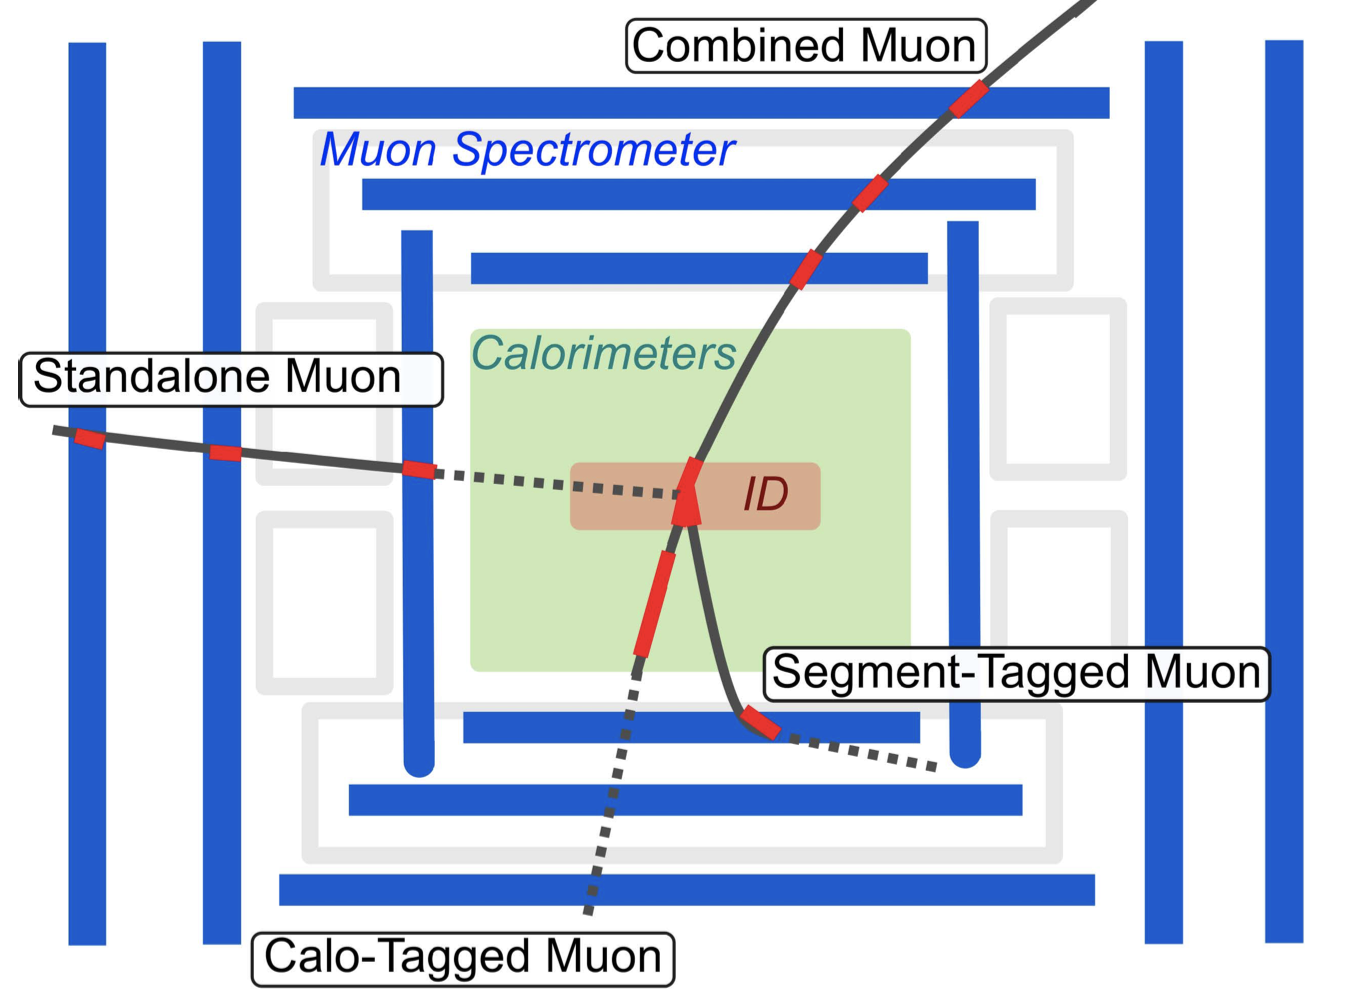
\includegraphics[width=0.8\linewidth]{figures//experiment/muonTypes.png}
    \caption{The different types of muons reconstructed by the ATLAS experiment.~\cite{Rettie:20188X}}
    \label{fig:muon-types}
\end{figure}


\Cref{fig:muon-steps} summarizes the steps used in the muon reconstruction for both the primary and the inside-out passes in ATLAS.

\begin{figure}[!ht]
    \centering
    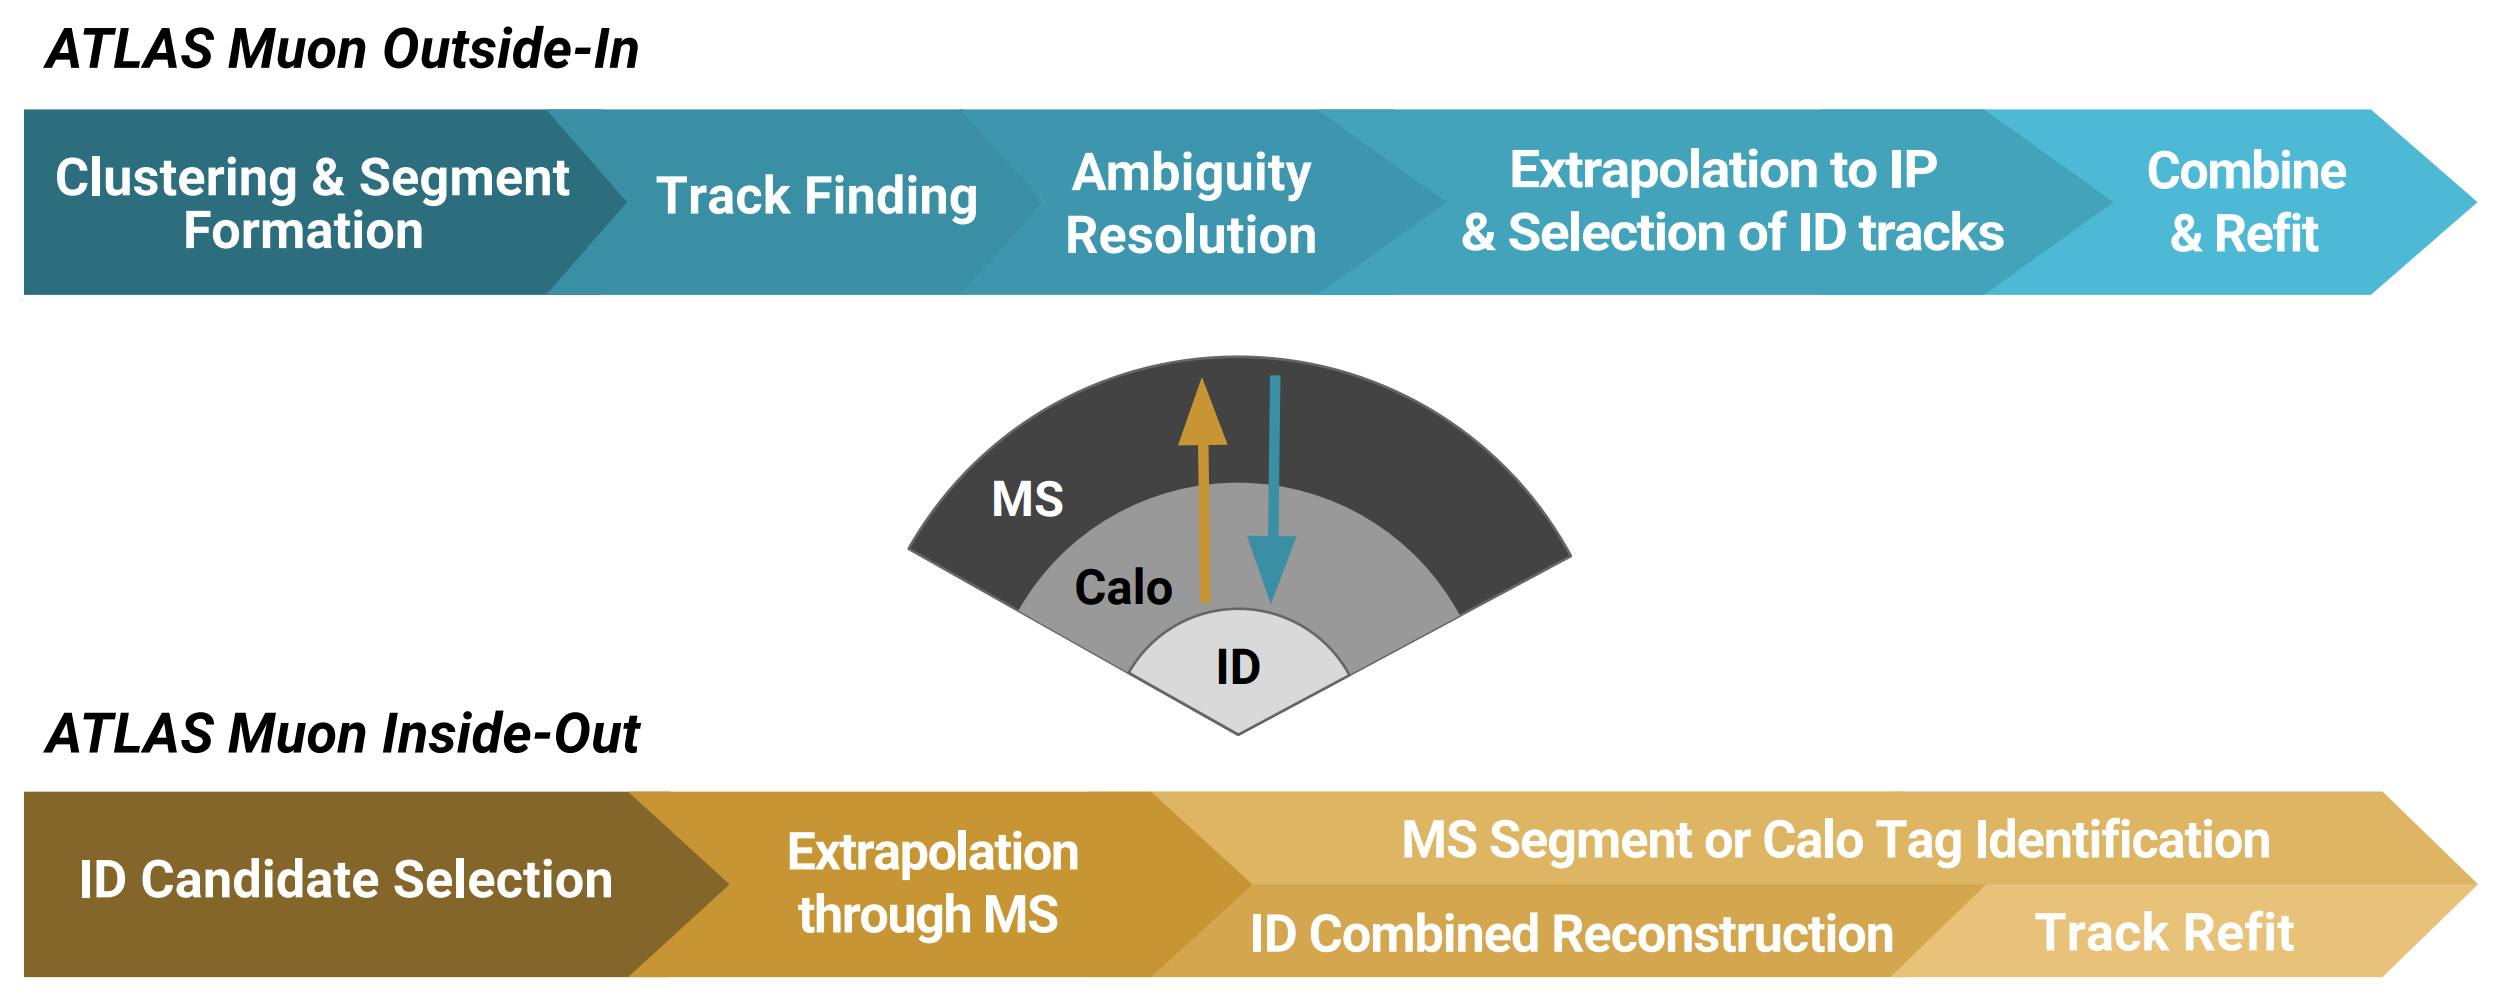
\includegraphics[width=0.8\linewidth]{figures//experiment/muonSteps.png}
    \caption{Simplified overview of the primary outside--in combined tracking chain and secondary inside--out chain used in ATLAS muon track reconstruction.~\cite{atlascollaboration2023software}}
    \label{fig:muon-steps}
\end{figure}

\subsection*{LRT Muons}
A dedicated muon reconstruction pass, functionally identical to the standard pass, is run using all the MS hits in an event along with LRT tracks (instead of the ID tracks from the standard passes) to gain sensitivity to LLP searches with muon final states. This reconstruction chain runs both \textit{outside-in} and \textit{inside-out}, however, only CB, ST, and CT muons are built using the LRT chain. The muons built from this pass are called LRT muons.

\subsection{Electrons}
Electrons in ATLAS are reconstructed using a combination of the ID and the calorimeters. Since electrons can lose a significant amount of their energy because of bremsstrahlung radiation, dedicated calorimetric reconstruction and track reconstruction methods are used to identify and reconstruct.~\Cref{fig:el-reco} provides a schematic illustration of the elements that enter into the reconstruction of an electron.


\begin{figure}[!ht]
    \centering
    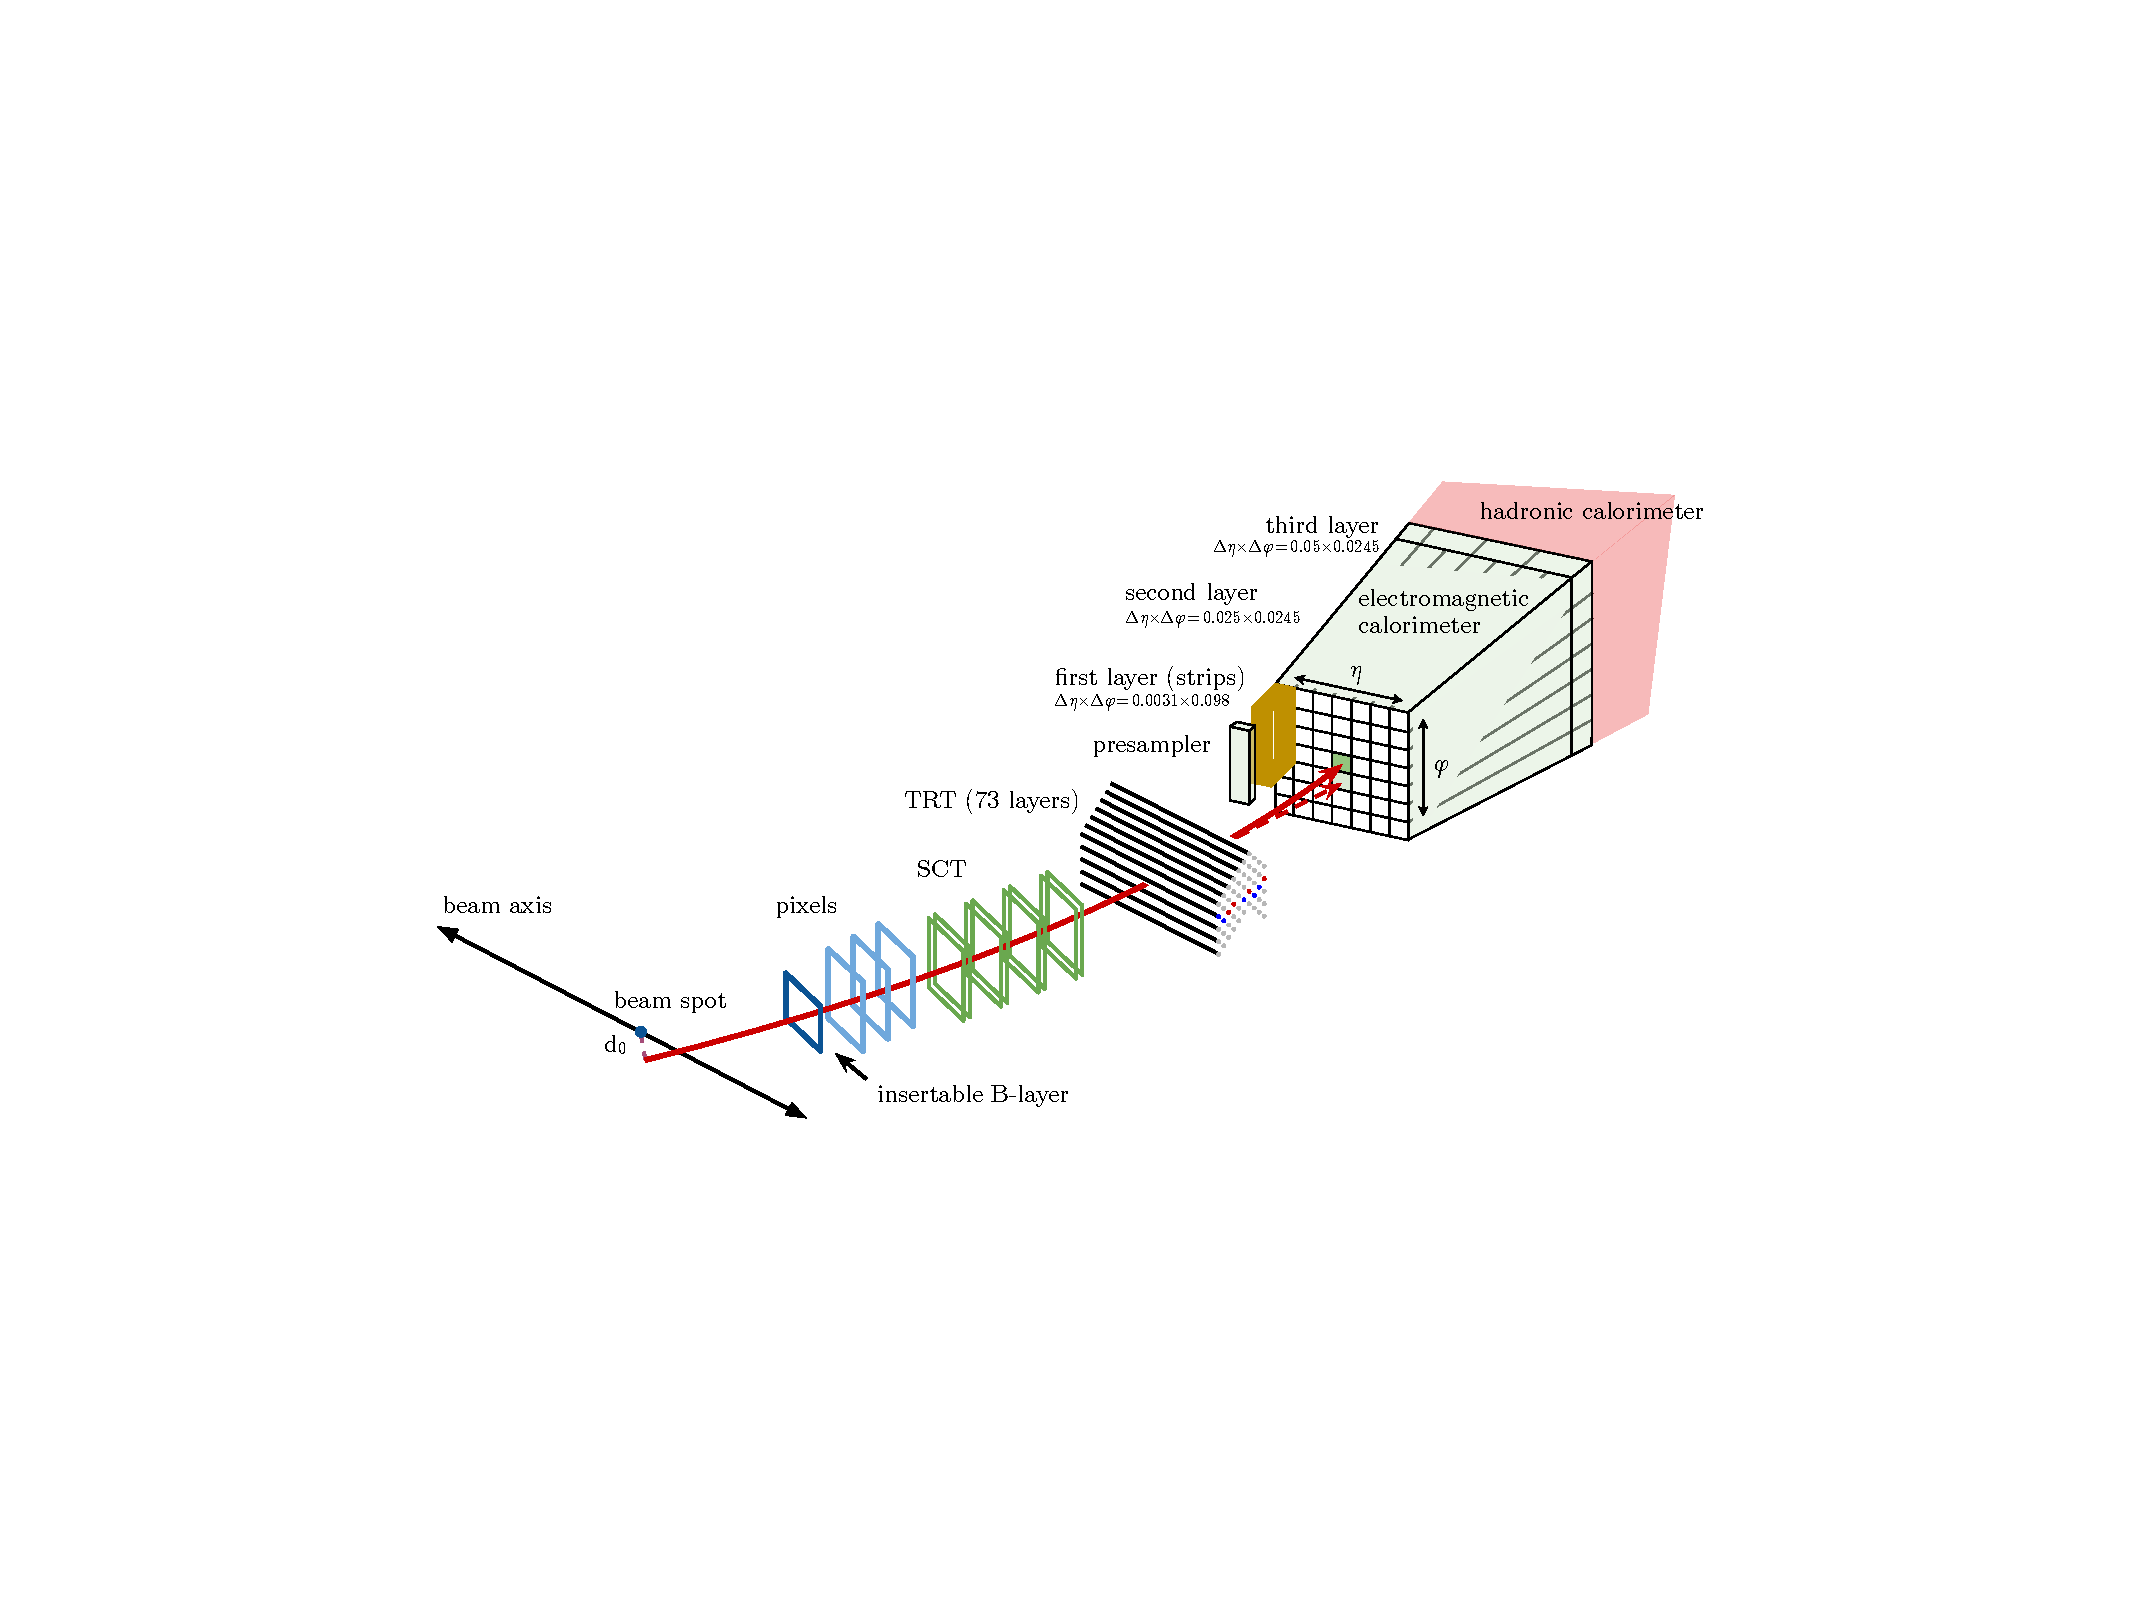
\includegraphics[width=0.8\linewidth]{figures//experiment/electronReco.pdf}
    \caption{A schematic illustration of the path of an electron through the detector. The red trajectory shows the hypothetical path of an electron, which first traverses the tracking system (pixel detectors, then silicon-strip detectors and lastly the TRT) and then enters the electromagnetic calorimeter. The dashed red trajectory indicates the path of a photon produced by the interaction of the electron with the material in the tracking system.~\cite{PERF-2017-01}}
    \label{fig:el-reco}
\end{figure}

The first step in electron reconstruction is seed-cluster formation. The three calorimeter layers and the pre-sampler are split into a grid in $\eta\times\phi$, and the energy deposited in each point (or \textit{tower}) in the grid is measured. Localized energy deposits are used to form electromagnetic-energy clusters. If two clusters share the same tower, the one with the higher energy is retained.

The second step in the reconstruction is track formation. Unlike MIPs, electrons interact strongly with the ID material and radiate photons. These decay products are expected to be highly collinear with the direction of the outgoing electron. A re-fit of the ID tracks is performed to build tracks for electron candidates allowing for energy losses up to 30\% due to bremsstrahlung using a Gaussian sum filter (GSF)~\cite{ATLAS-CONF-2012-047} designed to better account for energy loss of charged particles in material, is applied to the ID clusters of raw measurements. This procedure aims to recover tracks loosely matched to EM clusters. The GSF method accounts for radiative looses from electrons, and hence has a better $d_0$ resolution and $q/p$ accuracy for electrons than those from standard track reconstruction. The tracks built from this algorithm are called GSF tracks.

The last step in the reconstruction is the positional matching of the seed-clusters to the GSF tracks. Multiple ambiguity resolution steps are run to resolve tracks matched to the same clusters, as well as to differentiate genuine electron candidates from mis-identified photons. The energy of the electron is computed from the extended seed-cluster, while the directions are taken from the corresponding GSF track parameters.

\subsection*{LRT Electrons}
Similar to muons, a second reconstruction pass for non-pointing electrons is run using all the calorimeter clusters along with GSF tracks refit from LRT candidates (or LRT GSF tracks) to gain sensitivity to LLP searches with electron final states. The electrons built from this pass are called LRT electrons.

\subsection{Jets}
Jets are highly collimated showers of particles created by the rapid hadronization of quarks and gluons. The hadrons in the jets penetrate through the ECAL and are fully absorbed in the HCAL. Many algorithms exist for the reconstruction of jets, however, this analysis uses a particle flow implementation~\cite{PERF-2015-09} of the anti-$k_t$ algorithm~\cite{anti-kT}. This implementation uses information from the clusters in the calorimeter as well as hits in the ID to build jet objects with high energy and momentum resolution.

Anti-$k_t$ is a sequential recombination jet clustering algorithm, in which nearby\footnote{the \textit{closeness} of two particles or a particle and a pseudo-jet in this algorithm is determined by their transverse momenta, rapidities and azimuthal angles.} particles are iteratively collected and combined to form pseudo-jets. This process iterates over all set of particles available in the event till the \textit{size} of the pseudo-jet crosses a pre-defined distance metric (set to be 0.4 for the jets used in this analysis), at which point the pseudo-jet is deemed to be a jet~\cite{anti-kT}.

\begin{figure}[!ht]
    \centering
    
\includegraphics[width=\linewidth]{figures//experiment/pflowJets.png}
    \caption{A flow chart of how the particle flow algorithm proceeds, starting with track selection and continuing until the energy associated with the selected tracks has been removed from the calorimeter.~\cite{PERF-2015-09}}
    \label{fig:pflow}
\end{figure}

\Cref{fig:pflow} shows a schematic of the particle flow jet reconstruction algorithm used in ATLAS. Since tracks have better momentum resolution at lower \pT, and the calo-clusters have better energy resolution at high transverse energy deposits, the complementary information provided by the two sets of objects results in well-measured hadronic objects, where the ID is used for a measurement of the charged particle kinematics and the calorimeters provide information for the neutral particles. The particle flow algorithm provides a list of selected tracks and a list of topological-clusters (clusters of energy deposits in the calorimeters) containing initially unmodified clusters, as well as a new set-of clusters resulting from the energy subtraction procedure described in~\cref{fig:pflow}. In a case where a cluster and an ID track are matched to one another, the track measurement is used in place of the cluster, and its energy contribution is subtracted from the cluster to yield a modified cluster. Jets reconstructed from this full set of clusters and selected tracks are superior in terms of resolution and pileup robustness.